\documentclass{article}
\usepackage[top=0.75in, bottom=0.75in, left=1.25in, right=1in]{geometry} % formatage
\usepackage[frenchb]{babel}
\usepackage[utf8]{inputenc} 
\usepackage{amsmath} % pour utiliser des maths de base 
\usepackage{amssymb} % pour faire \mathcal{}=>des lettres ''cursives''
\usepackage{amsthm} % La petite boîte de fin de preuve
\usepackage{graphicx} % pour importer des images...http://www.tex.ac.uk/cgi-bin/texfaq2html?label=figurehere
\usepackage{titlesec} % automatique, pour faire des sous-titres moins laids
%\usepackage{cancel}
\usepackage[procnames]{listings}
\usepackage[T1]{fontenc}        % http://tex.stackexchange.com/questions/11897/draw-a-diagonal-arrow-across-an-expression-in-a-formula-to-show-that-it-vanishes%
\usepackage[squaren]{SIunits}
\usepackage{subcaption} % Avoir plusieurs sous-figures (graphiques) dans une figures et pouvoire les étiqueter
\usepackage{color}
\usepackage{lipsum}
\usepackage{caption}
\usepackage{enumitem} % Permet d'avoir plus de flexibilité dans les enumerations.
\usepackage{wasysym} 
\usepackage{braket}
\usepackage{mathtools}
\usepackage{multirow} % Fusionner des lignes dans un tableau
\usepackage{mathrsfs} % Faire le symbole de la transformée de Laplace
\usepackage{bbm}
\usepackage{array}
\usepackage{diagbox} % diagonale dans les tableaux
\usepackage{dsfont} % Faire des belles indicatrices                         
\usepackage{float} % placer les tableaux et images où tu veux
\usepackage{listings}
\usepackage[utf8]{inputenc}
\usepackage{comment}
\usepackage{pst-node}
\usepackage{fancyvrb} % Les varbatims gardent l'indentation
\usepackage{breakcites} % Faire en sorte que les citations ne sortent pas dans la marge
\usepackage{graphicx} % Insérer des graphiques
\usepackage{pgfplots}
\usepackage{hyperref} % Faire des hyperliens
\usepackage{verbatim} % Inclure un fichier .text en verbatim
\usepackage{xcolor}
\pgfplotsset{width=10cm, compat=1.9}

% Changer la couleur des hyperliens
\hypersetup{colorlinks = true,
	allcolors  = blue, % default color = black
	%	citecolor  = black
}  


% redefine \VerbatimInput
\RecustomVerbatimCommand{\VerbatimInput}{VerbatimInput}%
{fontsize=\footnotesize,
	%
	frame=lines,  % top and bottom rule only
	framesep=2em, % separation between frame and text
	rulecolor=\color{Gray},
	%
	label=\fbox{\color{Black}data.txt},
	labelposition=topline,
	%
	commandchars=\|\(\), % escape character and argument delimiters for
	% commands within the verbatim
	commentchar=*        % comment character
}


\newcommand{\RomanNumeralCaps}[1]
    {\MakeUppercase{\romannumeral #1}}

\newtheorem{lemme}{Lemme}
\newtheorem{preuve}{Preuve}
\newtheorem{code}{Code informatique}
\newtheorem{exemple}{Exemple}
\newtheorem{scenario}{Scénario}
\newtheorem{algo}{Algorithme}
\newtheorem{definition}{Définition}
\newtheorem{proposition}{Proposition}
\newtheorem{propriete}{Propriété}
\newtheorem{test_hypothese}{Teste d'hypothèse}

\begin{document}
	\renewcommand{\tablename}{Tableau}
	\renewcommand{\figurename}{Illustration}
	\renewenvironment{proof}{\noindent{\bfseries Démonstration.}}{\qed\\}
	\renewcommand{\natural}{\mathbb{N}}
	
	\newcommand{\VaR}{\mathrm{VaR}}
	\newcommand{\var}{\mathrm{Var}}
	\newcommand{\cov}{\mathrm{Cov}}
	\newcommand{\TVaR}{\mathrm{TVaR}}
	\newcommand{\E}{\mathbb{E}}
	\renewcommand{\P}{\mathbb{P}}
	\newcommand{\reel}{\mathbb{R}}
	
	\begin{titlepage}
		\centering % Centre everything on the title page
		
		\scshape % Use small caps for all text on the title page
		
		\vspace*{7\baselineskip} % White space at the top of the page
		
		%------------------------------------------------
		%	Title
		%------------------------------------------------
		
		\rule{\textwidth}{1.6pt}\vspace*{-\baselineskip}\vspace*{2pt} % Thick horizontal rule
		\rule{\textwidth}{0.4pt} % Thin horizontal rule
		
		\vspace{0.75\baselineskip} % Whitespace above the title
		{\LARGE Travail pratique 2\\} % Title
%		\vspace{0.75\baselineskip}
		\vspace{0.75\baselineskip} % Whitespace below the title
		
		\rule{\textwidth}{0.4pt}\vspace*{-\baselineskip}\vspace{3.2pt} % Thin horizontal rule
		\rule{\textwidth}{1.6pt} % Thick horizontal rule
		
		\vspace{4\baselineskip} % Whitespace after the title block
		
		%------------------------------------------------
		%	Subtitle
		%------------------------------------------------
		
		Travail présenté à \\
		{\scshape\Large M. Thierry Duchesne\\}
		
		\vspace*{4\baselineskip}
		
		Dans le cadre du cours\\
		{\scshape\Large Théorie et applications des méthodes de régression \\ STT-7125}
		
		% Subtitle or further description
		
		\vspace*{4\baselineskip} % Whitespace under the subtitle
		
		%------------------------------------------------
		%	Editor(s)
		%------------------------------------------------
		
		Réalisé par l'équipe 21:\\
		{\scshape\Large Alexandre Lepage\\
		\& Amedeo Zito} % Editor list
		
		\vspace*{5\baselineskip}
		
		le 17 décembre 2020
		
		\vspace{0.4\baselineskip} % Whitespace below the editor list
		
		\vfill % Whitespace between editor names and publisher logo
		
		%------------------------------------------------
		%	Publisher
		%------------------------------------------------
		
		
\includegraphics[height=1.2cm]{UL_P.pdf}\\
		
		Faculté des sciences et de génie\\
		École d'actuariat\\
		Université Laval
		
		\vspace*{3\baselineskip}
		
	\end{titlepage}
	
	\pagenumbering{Roman} % Pagination en chiffres romains
	\setcounter{page}{0} 
	
	\newpage
	\strut % Page blanche
	\newpage
	
	\tableofcontents
	\renewcommand{\listfigurename}{Liste des illustrations}
%	\newpage
	
	\listoffigures
%	\listoftables
	\newpage
	
	\pagenumbering{arabic} % Pagination en chiffres normaux
	\setcounter{page}{1}


\section*{Introduction}
Les modèles linéaires (LM) et modèles linéaires généralisés (GLM) sont des outils fort utiles pour modéliser toute sorte de phénomènes et sont largement utilisés dans le milieu statistique. Cependant, ces modèles s'appuient sur l'hypothèse que les observations $Y_1,\dots,Y_n,\ n>0$ servant à les entraîner sont indépendantes; laquelle n'est pas toujours réaliste selon le contexte.\\

Les modèles linéaires mixtes (LMM) permettent donc d'insérer une structure de dépendance entre les observations d'un LM. Du côté des GLM, il est possible d'effectuer un ajustement au modèle pour que la matrice de variance de celui-ci puisse tenir compte d'éventuelles covariances. De tels modèles ajustés sont appelés les GEE (\textit{Generalized Estimating Equation}).\\

L'objet de ce travail pratique est de mettre en pratique ces deux modèles. Ainsi, les questions 1 et 2 abordent le sujet des modèles linéaires mixtes tandis que la question 3 aborde le sujet des GEE.


\section{Modèle linéaire mixte pour les résultats en mathématique}\label{sect_qst1}
	Pour la première question de ce travail, on regarde les données d'un sous-ensemble des étudiants de 8ème année ayant participé au \textit{Nationnal Educationnal Longitudinal Study} de 1988. L'objectif de cette étude est de voir comment les résultats en mathématiques varient en fonction du nombre d'heures de travail à la maison (variable \texttt{homework} dans la base de données).
	Dans ce cas-ci, on a que la variable endogène $Y_{ij}$ correspond au résultat de l'examen de mathématique de l'étudiant $j$, appartenant à l'école $i$, $i=1,\dots, 23$, $j=1,\dots,n_i$, où $n_i$ correspond au nombre d'étudiants appartenant à la $i$-ème grappe. Dans la base de données, cette variable est désignée comme \texttt{math}.\\
	
	Comme la variable explicative \texttt{meanses}, correspondant au statut socio-économique moyen des étudiants de l’école, est fortement corrélée avec l'école d'origine des étudiants (variable de grappe), alors on est intéressé de voir quelle différence il y aurait entre un LMM avec et sans cette variable et de voir si le besoin d'effets aléatoires dans le modèle persiste si on ajoute cette dernière.

\renewcommand\thesubsection{\thesection\alph{subsection})}
\subsection{Exlusion de la variable \texttt{meanses}}\label{Qst1_a}
	Pour débuter l'entraînement d'un modèle, la première étape est de considérer un LM, d'évaluer ses résidus pour voir si les postulats sont respectés et de prendre action autrement. À noter que les LMM permettent de régler les problèmes d'auto-corrélation des résidus et, dans certains cas, de régler l'hétéroscédasticité.
	
	\subsubsection*{Entraînement d'un modèle linéaire}
		On considère le modèle linéaire suivant:
		\begin{align}\label{lm_1}
			Y_{ij} &= \beta_0 + \beta_1 \mathrm{homework} + \beta_2 \mathrm{white} + \beta_3 \mathrm{ratio} + \epsilon_{ij}.
		\end{align}
		Une analyse de multicolinéarité réalisée conformément à la méthodologie décrite dans le travail pratique 1 du présent cours ne soulève aucun problème. En revanche, lorsque l'on regarde l'illustration \ref{residus_VS_predicitions_lm1}, on voit que les résidus ont une légère tendance descendante. Le postulat de linéarité n'est donc pas respecté. Pour remédier à ce problème, on regarde les splines générés par un modèle additif généralisé (GAM) à l'aide de la fonction \texttt{gam} du \textit{package} du même nom. Ceux-ci sont présentés dans l'illustration \ref{Spline_lm1}.
		
		On voit donc dans l'illustration \ref{Spline_Homework} qu'il est possible de passer une droite dans l'intervalle de confiance entourant le spline. Pour cette variable, aucune transformation n'est donc nécessaire. Pour ce qui est de la variable \texttt{ratio}, il est impossible de passer une telle droite. Conséquemment, il faudrait ajouter un terme de deuxième degré sur la variable ratio qui aurait été centrée et réduite au préalable. Pour se faire, on pose
		$$ 
		\mathrm{ratio^*} = \frac{\mathrm{ratio}-18}{ \sigma_{\mathrm{ratio^*}}} 
		\quad\text{et}\quad
		\mathrm{ratio2} = (\mathrm{ratio^*})^2.
		$$
		Le modèle linéaire devient alors
		\begin{align}\label{lm_2}
				Y_{ij} &= \beta_0 + \beta_1 \mathrm{homework} + \beta_2 \mathrm{white} + \beta_3 \mathrm{ratio^*} + \beta_4 \mathrm{ratio2} + \epsilon_{ij}.
		\end{align}
		Si on refait l'exercice du GAM, on trouve l'illustration \ref{Spline_lm2}. Dans celle-ci, on remarque qu'aucune transformation additionnelle n'est nécessaire.
		Si on se fie à la statistique $F$ produite par la fonction \texttt{summary} en \texttt{R}, alors on trouve que la seule non-linéarité qui soit significative au seuil de 5\% est celle de la variable \texttt{homework}. Cependant, par soucis de simplicité, celle-ci ne sera pas modifiée. Par la suite, on peut tenter d'ajouter des interactions.
		Au seuil de 5\%, les interactions ajoutées sont \texttt{white:ratio} et \texttt{white:ratio2}, ce qui permet d'obtenir le modèle \eqref{lm_3}
		\begin{align}\label{lm_3}
			Y_{ij} &= \beta_0 + \beta_1 \mathrm{homework} + \beta_2 \mathrm{white} + \beta_3 \mathrm{ratio^*} + \beta_4 \mathrm{ratio2}\\
			 &+ \beta_5 (\mathrm{white:ratio^*}) + \beta_6 (\mathrm{white:ratio2}) + \epsilon_{ij}. \nonumber
		\end{align}
		
		L'illustration \ref{residus_VS_predicitions_lm3} permet de voir que la linéarité semble meilleure, mais que le problème est désormais au niveau de l'hétéroscédasticité des résidus. Or, un LMM peut aider à traiter ce genre de problème. Du point de vue de l'auto-corrélation des observations du jeu de données, l'illustration \ref{residus_VS_id_qst1a} permet de voir que, selon l'école d'appartenance des élèves, les résidus du LM ne sont pas identiquement distribués. En effet, selon la grappe, on voit que les résidus ont une variance et une moyenne qui peut différer. Cette observation vient donc légitimer l'utilisation d'un LMM.
		
	\subsubsection*{Entraînement d'un modèle linéaire mixte}
		Maintenant qu'un modèle linéaire a été entraîné et que l'on a observé la nécessité d'y inclure des effets aléatoires pour tenir compte de la corrélation qui existe entre les élèves d'une même école, il est temps d'entraîner un LMM.\\
		
		Pour se faire, la première étape est de faire les graphiques des résidus en fonction des différentes variables pour voir sur lesquelles d'entre elles il serait intéressant appliquer un effet aléatoire. Bien que cela soit difficile à voir, l'illustration \ref{Residus_VS_variables_lm3} montre que la variable la plus susceptible d'avoir un effet aléatoire est \texttt{homework} puisqu'elle est celle ayant le plus de volatilité dans la distribution des résidus selon les valeurs qu'elle peut prendre. Ainsi, avec la fonction \texttt{lmer} du \texttt{package R lme4}, on entraîne le modèle \eqref{lmm_1} avec les structures de variance VC\footnote{\textit{Variance Components}: indépendance entre les termes de résidus.} pour la variance des résidus et UN\footnote{\textit{Unstructured}: il existe une corrélation entre les effets aléatoires.}, de même que UN(1)\footnote{\textit{Diagonales principales}: les effets aléatoires sont indépendants l'un de l'autre.} pour la variance des effets aléatoires.
		\begin{align}\label{lmm_1}
			Y_{ij} &= \beta_0+\gamma_{i0} + (\beta_1 + \gamma_{i1}) \mathrm{homework} + \beta_2 \mathrm{white} + \beta_3 \mathrm{ratio^*} \\
			&+ \beta_4 \mathrm{ratio2} + \beta_5( \mathrm{white:ratio^*}) + \beta_6 (\mathrm{white:ratio2}) + \epsilon_{ij}. \nonumber
		\end{align}
		À noter que l'ajout de trop d'effets aléatoires dans le modèle testé peut entraîner de l'instabilité numérique lors de l'entraînement de celui-ci. C'est pourquoi on se limite à deux effets aléatoires dans le modèle \eqref{lmm_1}.\\
		
		En ce qui attrait à la structure de variance des résidus de type CS\footnote{\textit{Compound symmetry}: la corrélation entre les résidus est la même partout.}, comme la fonction \texttt{lmer} ne permet pas de l'utiliser, on peut faire appel à la fonction \texttt{lme} du \textit{package} \texttt{nlme}.
		%
		Pour ce qui est de la structure AR(1)\footnote{\textit{Auto-régression d'ordre 1}: la corrélation diminue selon un aspect d'éloignement (généralement pour les observations qui sont étudiées à travers le temps ou l'espace).}, celle-ci n'a que peu de sens dans ce contexte puisque les observations (les élèves d'une même école) ne peuvent pas être ordonnées selon un ordre chronologique ou spatial. Pour cette raison, on ne considérera pas cette dernière.\\

		Comme les trois modèles testés possèdent tous la même composante fixe ($\boldsymbol{X\beta}$), alors on peut comparer les log-vraisemblances de même que les AIC. Le tableau \ref{tbl_AIC_Qst1a} présente donc l'AIC pour chacun des modèles testés.
		\begin{table}[H]
			\centering
			\begin{tabular}{ll|rr}
				\hline
				$\var(\boldsymbol{\epsilon})$ & $\var(\boldsymbol{\gamma})$ & $dl$ & AIC \\ 
				\hline
				VC & UN & 11.00 & 3630.72 \\ 
				VC & UN(1) & 10.00 & 3658.96 \\ 
				CS & UN & 12.00 & 3621.86 \\
				\hline
			\end{tabular}
		\caption{AIC des trois modèles testés en fonction de \eqref{lmm_1} avec le nombre de degrés de liberté $dl$ associé à chacun d'eux.}
		\label{tbl_AIC_Qst1a}
		\end{table}
		Avec le tableau \ref{tbl_AIC_Qst1a}, on voit que la structure de variance qui minimise l'AIC est CS/UN. Cependant, avec la fonction \texttt{summary} de \texttt{R}, on voit que le coefficient de corrélation des résidus d'une même classe est de $5.126496\times10^{-18}$, ce qui est très près de zéro. On peut donc simplifier le modèle et prendre la structure VC/UN.
		Puis on voit que la corrélation entre les effets aléatoires $\gamma_{i0}$ et $\gamma_{i1}$ est de -0.89, ce qui confirme qu'il existe un lien de dépendance significatif entre ces variables aléatoires et que la structure de variance UN est approprié.
		%
		En somme, la corrélation entre les étudiants d'une même école est négligeable et il existe un lien de dépendance significatif entre les effets aléatoires du modèle.\\
		
		Après avoir sélectionné les structures de variance du LMM, il faut tester si les effets aléatoires du modèle \eqref{lmm_1} sont nécessaires. Pour se faire, il s'agit de procéder à un test du ratio des vraisemblances. 
		Soit les hypothèses de test suivantes:
		\begin{align*}
			H_0: &\text{ Le modèle simple est suffisant;}\\
			H_1: &\text{ Le modèle complet représente mieux les données.}
		\end{align*}
		Soit $l_0$ et $l_1$, la log-vraisemblance sous $H_0$ et celle sous $H_1$. On définit  $\Delta_{dl}$ comme la différence du nombre de paramètres entre les deux modèles.
		Le calcul de la \textit{$p$-value} du test est effectué avec \eqref{eq_LRT}.
		\begin{equation}\label{eq_LRT}
			p\mathrm{-value} = 0.5\left[2- \P(\chi^2_{\Delta_{dl} - 1} > \xi) - \P(\chi^2_{\Delta_{dl}} > \xi)\right],
		\end{equation} 
		On applique ainsi \eqref{eq_LRT} pour évaluer si l'effet aléatoire $\gamma_{i1}$ est significatif et on trouve une statistique de test de 92.92 avec $\Delta_{dl}=2$, ce qui permet de calculer un seuil observé de 0. Conséquemment, on rejette fortement $H_0$ et on conserve l'effet aléatoire $\gamma_{i1}$. De plus, puisque $\gamma_{i1}$ est conservé, on ne peut retirer l'ordonnée à l'origine aléatoire. Le modèle obtenu suite à cette étape de construction du LMM correspond ainsi à \eqref{lmm_2}.
		\begin{align}\label{lmm_2}
			Y_{ij} &= \beta_0+\gamma_{i0} + (\beta_1 + \gamma_{i1}) \mathrm{homework} + \beta_2 \mathrm{white} + \beta_3 \mathrm{ratio^*} \\
			&+ \beta_4 \mathrm{ratio2} + \beta_5 (\mathrm{white:ratio^*}) + \beta_6 (\mathrm{white:ratio2}) + \epsilon_{ij}. \nonumber
		\end{align}
		
		Il ne reste plus qu'à sélectionner les effets fixes. Pour se faire, on utilise le test de Wald de type III utilisé par la fonction \texttt{Anova} du \textit{package} \texttt{car}.
		%
		On remarque alors que la variable \texttt{ratio}$^*$ possède un seuil de test de 15.69\%. Cependant, comme on ne peut la retirer sans avoir retiré les variables dépendantes d'elle au préalable, c.-à-d. \texttt{white:ratio2}, \texttt{white:ratio}$^*$ et \texttt{ratio2}, on ne peut pas l'enlever. Conséquemment, on va commencer par retirer l'interaction \texttt{white:ratio2} avant de réeffectuer le test. Puis, on retire aussi \texttt{white:ratio}$^*$ puisque la variable \texttt{ratio}$^*$ n'est toujours pas significative au seuil de 5\%. On fait de même avec \texttt{ratio2} pour finalement retirer \texttt{ratio}$^*$. On trouve ainsi le modèle final \eqref{lmm_qst1a}.
		\begin{align}\label{lmm_qst1a}
			Y_{ij} = \beta_0+\gamma_{i0} + (\beta_1 + \gamma_{i1}) \mathrm{homework} + \beta_2 \mathrm{white} + \epsilon_{ij}.
		\end{align}
		Avec la fonction \texttt{summary} de \texttt{R}, on obtient les résultats présentés dans l'illustration \ref{summary_Qst1a}. D'une part, on a les effets fixes pour lesquels un intervalle de confiance à 95\% est calculé dans le tableau \ref{tbl_effets_fixes_qst1a}.
		\begin{table}[H]
			\centering
			\begin{tabular}{lrrrr}
				\hline
				& Estimateur & Écart-type & \multicolumn{2}{c}{IC 95\%} \\ 
				\hline
				$\beta_0$ & 44.02 & 1.83 & 40.42 & 47.62 \\ 
				$\beta_1$ & 1.90 & 0.92 & 0.11 & 3.70 \\ 
				$\beta_2$ & 3.30 & 0.98 & 1.38 & 5.22 \\ 
				\hline
			\end{tabular}
		\caption{Estimateurs des poids pour les effets fixes du LMM ainsi que leurs intervalles de confiance à 95\%.}
		\label{tbl_effets_fixes_qst1a}
		\end{table}
		%
		D'autre part, on a 
		\begin{align}
			\boldsymbol{D}_i = \var(\boldsymbol{\gamma}_i) = 
			\begin{bmatrix}
				58.20797 & -27.01225 \\
				-27.01225& 17.25707  \\
			\end{bmatrix},
			i=1,\dots,23
			%
			\; \text{ et }\;
			\boldsymbol{D} = 
			\begin{bmatrix}
				D_1 & 0 & \dots & 0 \\
				0 & D_2 & 0 & \vdots \\
				\vdots & 0 & \ddots & 0 \\
				0 & \dots & 0 & D_{23}
			\end{bmatrix}
		\end{align}
		De plus,
		\begin{align}
			\boldsymbol{V} = \var(\boldsymbol{\epsilon}) = 
			52.66\, \boldsymbol{I}_{n\times n},
			\ n=\sum_{i=1}^{23} n_i = 519.
		\end{align}
	
		
	\subsubsection*{Discussion}
		Avec le tableau \ref{tbl_effets_fixes_qst1a}, on voit que, toute autre chose étant égale, chaque heure de travail supplémentaire à la maison contribue à augmenter la note moyenne d'un étudiant pour son examen de mathématique de 1.90\%. Cet effet est significatif puisque l'intervalle de confiance à 95\% de l'estimateur n'inclut pas la valeur 0. Par ailleurs, comme on a pu l'observer lors de l'étape du test des effets aléatoires, l'effet du nombre d'heures de travail à la maison peut varier d'une école à l'autre.
		
\subsection{Inclusion de la variable \texttt{meanses}}\label{Qst1_b}
	Comme pour la partie \ref{Qst1_a}, on commence par entraîner un modèle linéaire mixte et on procède de façon similaire pour trouver le modèle \eqref{lm_qst1b}.
	\begin{align}\label{lm_qst1b}
		Y_{ij} &= \beta_0 + \beta_1 \mathrm{meanses} + \beta_2\mathrm{homework} + \beta_3\mathrm{white} + \beta_4\mathrm{ratio^*} + \beta_5\mathrm{ratio2} \\
		&+ \beta_6(\mathrm{white:ratio}) + \beta_7(\mathrm{white:ratio2}) + \beta_8(\mathrm{meanses:white}) + \beta_9(\mathrm{meanses:ratio2}) + \epsilon_{ij}.\nonumber
	\end{align}
	À noter que l'interaction des variables \texttt{homework} et \texttt{meanses} n'est pas significatif au seuil de 5\%.\\
	
	En comparant les illustrations \ref{residus_VS_id_qst1a} et \ref{residus_VS_id_qst1b}, on voit que l'ajout de la variable \texttt{meanses} au modèle semble, a priori, régler le problème de corrélation entre les observations. En effet, on voit dans l'illustration \ref{residus_VS_id_qst1b} que les résidus de chacune des écoles semblent centrées à zéro. Cependant les variance varient encore quelque peu. Voyons maintenant si l'ajout d'effets aléatoires serait significatif.
	\subsubsection*{Entraînement d'un modèle linéaire mixte} 
		Pour débuter,  l'illustration \ref{Residus_VS_variables_qst1b}
		montre que, encore une fois, seule la variable \texttt{homework} est susceptible de recevoir un effet aléatoire. Afin de confirmer cette observation, on peut entraîner un LMM ne comportant que deux effets aléatoires, soit une ordonnée à l'origine et un effet sur l'une des variables explicatives parmi \texttt{homework}, \texttt{meanses} et \texttt{ratio}$^*$.
		On teste ainsi chacune des variables avec les trois structures mentionnées ci-haut, soit VC/UN, VC/UN(1) et CS/UN. Il en découle que le modèle qui minimise l'AIC, est celui incluant un effet aléatoire à la variable \texttt{homework}. Par la suite, si on tente d'ajouter un troisième effet aléatoire, on obtient que les fonctions \texttt{lmer} et \texttt{lme} deviennent instables numériquement. On s'en tiendra donc à 2 effets. En ce qui attrait aux structures de variances, celle qui minimise l'AIC est la structure CS/UN. Cependant, comme dans la section \ref{Qst1_a}, on a un coefficient de corrélation pour la variance de $\boldsymbol{\epsilon}_i$ qui est de $5.126496\times 10^{-18}$. La dépendance entre les résidus d'une même grappe est donc négligeable et on peut simplifier le modèle en adoptant la structure VC/UN. Plus encore, la corrélation entre l'ordonnée à l'origine aléatoire et l'effet appliqué à la variable \texttt{homework} est de -0.91 confirmant ainsi que la structure UN est adéquate pour la variance de $\boldsymbol{\gamma}$.\\
		
		Par la suite, on effectue le test du ratio des vraisemblances dont le calcul du seuil observé est présenté en \eqref{eq_LRT}. On trouve ainsi une statistique de test de 90.95 avec $\Delta_{dl}=2$, pour un seuil observé de 0. L'évidence est donc forte contre l'hypothèse nulle et on peut en conclure que l'effet aléatoire ajouté à la variable \texttt{homework} est significatif.\\
		
		Pour ce qui est de la sélection des effets fixes, on a que la variable ayant le plus grand seuil observé avec le test de Wald de type III est \texttt{ratio}$^*$. Cependant, comme pour la section \ref{Qst1_a}, on doit gérer les variables d'ordre supérieur qui dépendent de celle-ci avant de pouvoir la retirer. On commence donc par retirer l'interaction \texttt{white:ratio2}. Puis, on refait le test pour retirer \texttt{ratio2}; ainsi de suite jusqu'à trouver le modèle \eqref{lmm_qst1b} où tous les effets fixes sont significatifs au seuil de 5\%.
		\begin{equation}\label{lmm_qst1b}
			Y_{ij} = \beta_0 + \gamma_{i0} + \beta_1 \mathrm{meanses} + (\beta_2 + \gamma_{i2}) \mathrm{homework} + \beta_3\mathrm{white} + \epsilon_{ij}.
		\end{equation}
		Si on essaie d'intégrer l'interaction \texttt{meanses:homework}, on trouve un seuil de test de 0.7368; on ne l'inclue donc pas dans le modèle.		
		La sortie \texttt{R} de la fonction \texttt{summary} appliquée sur le modèle ainsi obtenu est présentée dans l'illustration \ref{summary_Qst1b}. Les effets fixes sont décrits dans le tableau \ref{tbl_effets_fixes_qst1b} et les matrices de variances sont présentées dans \eqref{matrice_D_qst1b} et \eqref{matrice_V_qst1b}, lesquelles sont exactement les mêmes que dans la section \ref{Qst1_a}.
		\begin{table}[ht]
			\centering
			\begin{tabular}{lrrrr}
				\hline
				& Estimateurs & Écarts-types &  \multicolumn{2}{c}{IC 95\%} \\ 
				\hline
				$\beta_0$ & 44.70 & 1.79 & 41.20 & 48.21 \\ 
				$\beta_1$ & 4.89 & 1.34 & 2.26 & 7.52 \\ 
				$\beta_2$ & 1.93 & 0.90 & 0.17 & 3.68 \\ 
				$\beta_3$ & 3.11 & 0.96 & 1.24 & 4.99 \\ 
				\hline
			\end{tabular}
		\caption{Estimateurs des poids pour les effets fixes du LMM \eqref{lmm_qst1b} ainsi que leurs intervalles de confiance à 95\%.}
		\label{tbl_effets_fixes_qst1b}
		\end{table}
		%
		\begin{align}\label{matrice_D_qst1b}
			\boldsymbol{D}_i = \var(\boldsymbol{\gamma}_i) = 
			\begin{bmatrix}
				58.20797 & -27.01225 \\
				-27.01225& 17.25707  \\
			\end{bmatrix},
			i=1,\dots,23
			%
			\; \text{ et }\;
			\boldsymbol{D} = 
			\begin{bmatrix}
				D_1 & 0 & \dots & 0 \\
				0 & D_2 & 0 & \vdots \\
				\vdots & 0 & \ddots & 0 \\
				0 & \dots & 0 & D_{23}
			\end{bmatrix}
		\end{align}
		%
		\begin{align}\label{matrice_V_qst1b}
			\boldsymbol{V} = \var(\boldsymbol{\epsilon}) = 
			52.66\, \boldsymbol{I}_{n\times n},
			\ n=\sum_{i=1}^{23} n_i = 519.
		\end{align}
	\subsubsection*{Discussion}
		Comme on a pu l'observer avec l'illustration \ref{residus_VS_id_qst1b}, l'ajout de la variable \texttt{meanses} qui est très fortement corrélée avec les identifiants des écoles (les grappes) a réduit considérablement le besoin d'ajouter des effets aléatoires au modèle puisque les résidus sont maintenant centrés autour de zéro. Néanmoins, avec le test du ratio des vraisemblances, on a pu voir que l'effet aléatoire appliqué à la variable \texttt{homework}, de même que l'ordonnée à l'origine aléatoire, sont utiles.\\
		
		Au final, on trouve que l'ajout d'une heure supplémentaire d'étude augmente, en moyenne, l'espérance de la note en mathématique de 1.925\% et cet effet varie d'une école à l'autre (effet aléatoire).
	
\section{Modèle linéaire mixte pour la grandeur de jeunes filles}
	Pour cette deuxième question, le jeu de données à l'étude présente 20 courbes de la croissance de jeunes filles mesurées annuellement entre les âges 6 à 10 ans. Celui-ci a été publié par Gildstein (1979). Dans ce cas-ci, la variable endogène $Y_{ij}$ correspond à la taille de la $i-ème$ fille lors de sa $j$-ème mesure à l'âge $5+j$, $i=1,\dots,20,\ j=1,\dots,5$.
	
	\subsubsection*{Entraînement d'un modèle linéaire}
		Afin de voir si la relation qui existe entre l'âge des petites filles et leur grandeur est linéaire, on regarde l'illustration \ref{Grandeur_VS_age_Qst2}. Comme celle-ci l'est effectivement, on entraîne le modèle \eqref{lm_qst2_1}.
		\begin{equation}\label{lm_qst2_1}
			Y_{ij} = \beta_0 + \beta_1 \mathrm{age} + \beta_2 \mathrm{group_2} + \beta_3 \mathrm{group_3} + \beta_4 (\mathrm{group_2:age}) + \beta_5 (\mathrm{group_3:age}) + \epsilon_{ij}.
		\end{equation}
		Comme \eqref{lm_qst2_1} possède un facteur d'inflation de la variance généralisé ($\mathrm{GVIF}_j^{1/(2p_j)}$) supérieur à $\sqrt{10} = 3.16$, on est en présence de multicolinéarité. Pour remédier à ce problème, on peut simplement tronquer la variable \texttt{age} de la manière suivante:
		$$\mathrm{temps}=\mathrm{age}-6.$$
		Le modèle \eqref{lm_qst2_1} devient alors \eqref{lm_qst2}.
		\begin{equation}\label{lm_qst2}
			Y_{ij} = \beta_0 + \beta_1 \mathrm{temps} + \beta_2 \mathrm{group_2} + \beta_3 \mathrm{group_3} + \beta_4 (\mathrm{group_2:temps}) + \beta_5 (\mathrm{group_3:temps}) + \epsilon_{ij}.
		\end{equation}
		Avec ce dernier, on calcule les résidus studentisés de manière à générer l'illustrations \ref{residus_qst2}. Dans un premier temps, on remarque avec l'illustration \ref{residus_VS_id_qst2} que les résidus ne sont pas tous centrés autour de zéro. Dépendamment de la fillette, ceux-ci ont une moyenne qui diffère grandement, ce qui laisse présager une corrélation entres les observations d'une même fillette. Cela suggère qu'un LMM pourrait régler le problème d'auto-corrélation des résidus.
		
		\subsubsection*{Entraînement d'un modèle linéaire mixte}
		Dans un deuxième temps, on remarque avec les illustrations \ref{residus_VS_id_qst2} et \ref{Residus_VS_temps_qst2} que les deux graphiques sont pratiquement identiques, laissant présager qu'un effet aléatoire sur la variable \texttt{temps} n'aurait aucune incidence sur les résidus. Plus encore, avec l'illustration \ref{Residus_VS_group_qst2}, on voit que les résidus varient énormément selon la valeur de la variable \texttt{group}. Cela pourrait expliquer en partie les ordonnées à l'origine des résidus qui diffèrent dans \ref{residus_VS_id_qst2}.\\		
	
		Voyons maintenant si ces observations s'avèrent réalistes en entraînant un LMM avec les structures de variances VC/UN, CS/UN et AR(1)/UN. À noter que la structure AR(1) pour la variance des résidus est particulièrement intéressante dans ce contexte puisque les observations d'une même fillettes peuvent être ordonnées chronologiquement.
		%
		À cet effet, avec ce dernier, l'ajout de la variable \texttt{temps} dans les effets aléatoires engendre des problèmes de convergence avec la fonction \texttt{lme}. Conséquemment, le modèle entraîné à cette étape consiste en \eqref{lmm_qst2_1}.
		\begin{align}\label{lmm_qst2_1}
			Y_{ij} &= \beta_0 + \gamma_{i0} + \beta_1 \mathrm{temps} + (\beta_2 + \gamma_{i2}) \mathrm{group_2} \\
			&+ (\beta_3 + \gamma_{i3}) \mathrm{group_3} + \beta_4 (\mathrm{group_2:temps}) + \beta_5 (\mathrm{group_3:temps}) + \epsilon_{ij}. \nonumber
		\end{align}
		L'AIC calculé pour chacun des modèles entraîné est présenté dans le tableau \ref{tbl_AIC_Qst2}
		\begin{table}[H]
			\centering
			\begin{tabular}{ll|rr}
				\hline
				$\var(\boldsymbol{\epsilon})$ & $\var(\boldsymbol{\gamma})$ & $dl$ & AIC \\ 
				\hline
				VC & UN & 13.00 & 356.72 \\ 
				CS & UN & 14.00 & 360.87 \\ 
				AR(1) & UN & 14.00 & 336.09 \\ 
				\hline
			\end{tabular}
			\caption{AIC des trois modèles testés en fonction de \eqref{lmm_qst2_1} avec le nombre de degrés de liberté $dl$ associé à chacun d'eux.}
			\label{tbl_AIC_Qst2}
		\end{table}
	On voit avec le tableau \ref{tbl_AIC_Qst2} que la structure de variance la plus appropriée selon le critère de l'AIC pour le modèle \eqref{lmm_qst2_1} est AR(1)/UN. Plus encore, le coefficient de corrélation liant les résidus d'une même fillette est de 0.9041, ce qui est hautement significatif. De plus, la matrice des coefficients de corrélation des effets aléatoire s'exprime comme
	$$
		\boldsymbol{\rho}(\boldsymbol{\gamma}_i) = 
		\begin{bmatrix}
			1 & 0.380 & -0.147 \\
			0.380 & 1 & -0.813 \\
			-0.147 & -0.813 & 1
		\end{bmatrix},\ i=1,\dots, 20.
	$$
	Ainsi, la structure de variance non structurée (UN) est justifiée pour les effets aléatoires puisque les coefficients de corrélations sont significativement différents de zéro.\\
	
	Si on fait un test du ratio des vraisemblances pour l'effet aléatoire appliqué sur la variable \texttt{group}, on trouve une statistique de test de 1.39 pour $\Delta_{dl}=5$, ce qui donne un seuil observé de 0.885. Ainsi, on ne peut rejeter l'hypothèse nulle que l'effet aléatoire associé à la variable \texttt{group} n'est pas significatif et on peut le retirer. Si on refait le test sur l'ordonnée à l'origine aléatoire, on trouve une statistique de 185.54 pour $\Delta_{dl}=2$, ce qui donne un seuil observé de 0. On ne peut donc pas retirer l'ordonnée à l'origine aléatoire. Mentionnons que pour ce dernier test, comme on compare un modèle linéaire ($H_0$) à un modèle mixte ($H_1$), on ne peut utiliser la méthode REML pour calculer la log-vraisemblance de ce dernier lors du test puisque le modèle linéaire associé à l'hypothèse nulle utilise le maximum de vraisemblance.\\
	
	Au niveau des effets fixes, le test de Wald de type III indique que tous les effets fixes sont significatifs au seuil de 5\%. On obtient donc le modèle final \eqref{lmm_qst2_final}
	\begin{align}\label{lmm_qst2_final}
		Y_{ij} &= \beta_0 + \gamma_{i0} + \beta_1 \mathrm{temps} + \beta_2 \mathrm{group_2} + \beta_3 \mathrm{group_3}\\
		&+ \beta_4 (\mathrm{group_2:temps}) + \beta_5 (\mathrm{group_3:temps}) + \epsilon_{ij}. \nonumber
	\end{align}
	La sortie \texttt{R} de la fonction \texttt{summary} appliquée sur le modèle ainsi obtenu est présentée dans l'illustration \ref{summary_Qst2}. Les effets fixes sont décrits dans le tableau \ref{tbl_effets_fixes_qst2} et les matrices de variances sont présentées dans \eqref{matrices_D_qst2} et \eqref{matrices_V_qst2}.
	\begin{table}[ht]
		\centering
		\begin{tabular}{lrrrr}
			\hline
			& Estimateurs & Écarts-types &  \multicolumn{2}{c}{IC 95\%} \\ 
			\hline
			$\beta_0$ & 112.57 & 1.22 & 110.18 & 114.96 \\ 
			$\beta_1$ & 3.70 & 1.66 & 0.44 & 6.96 \\ 
			$\beta_2$ & 7.79 & 1.66 & 4.54 & 11.05 \\ 
			$\beta_3$ & 5.29 & 0.19 & 4.92 & 5.65 \\ 
			$\beta_4$ & 0.26 & 0.25 & -0.23 & 0.76 \\ 
			$\beta_5$ & 0.87 & 0.25 & 0.37 & 1.37 \\ 
			\hline
		\end{tabular}
		\caption{Estimateurs des poids pour les effets fixes du LMM \eqref{lmm_qst2_final} ainsi que leurs intervalles de confiance à 95\%.}
		\label{tbl_effets_fixes_qst2}
	\end{table}
	%
	\begin{equation}\label{matrices_D_qst2}
		\boldsymbol{D} = 5.088543\times10^{-6}\, \boldsymbol{I}_{20\times 20}
	\end{equation}
	et
	\begin{equation}\label{matrices_V_qst2}
		\boldsymbol{V}_i = 
		\begin{bmatrix}
			2.988 & 2.838 & 2.696 & 2.560 & 2.432 \\
			2.838 & 2.988 & 2.838 & 2.696 & 2.560 \\
			2.696 & 2.838 & 2.988 & 2.838 & 2.696 \\
			2.560 & 2.696 & 2.838 & 2.988 & 2.838 \\
			2.432 & 2.560 & 2.696 & 2.838 & 2.988
		\end{bmatrix}, \ i=1,\dots,20,\ 
	\boldsymbol{V} = \begin{bmatrix}
		V_1 & 0 & \dots & 0 \\
		0 & V_2 & 0 & \vdots \\
		\vdots & 0 & \ddots & 0 \\
		0 & \dots & 0 & V_{20}
	\end{bmatrix}
	\end{equation}
			
	\subsubsection*{Discussion}
		L'interprétation des résultats obtenus dans le tableau \ref{tbl_effets_fixes_qst2} est synthétisée dans le tableau \ref{tbl_interpretation_qst2}.
		\begin{table}[H]
			\centering
			\begin{tabular}{lccc}
				\hline
				Taille de  & Taille de la  & Taux de croissance  &  Grandeur de la \\
				la mère & fille à 6 ans & annuel &  fille à 10 ans \\
				\hline
				petite & 112.57 & 3.70 & 127.37 \\
				moyenne & 120.36 & 3.96 & 136.20 \\
				grande & 117.86 & 4.57 & 136.14 \\
				\hline
			\end{tabular}
			\caption{Mesures moyennes(en cm) pour une petite fille qui est née en 1973 selon la grandeur de la mère.}
			\label{tbl_interpretation_qst2}
		\end{table}
		Avec la matrice $\boldsymbol{D}$ obtenue en \eqref{matrices_D_qst2}, on voit que l'effet aléatoire tend à être dégénérée puisque sa variance tend vers zéro. En somme, on peut résumer l'effet aléatoire $\gamma_{i0}$ comme une constante, soit 0. Néanmoins, le modèle mixte est utile puisqu'il fait un ajustement sur la variance des prévisions pour tenir compte de la corrélation entre les mesures d'une même petite fille.
		On a donc $\boldsymbol{Y}_{i} \sim N(\boldsymbol{X}_{i}'\boldsymbol{\beta}, \boldsymbol{V}_i)$ où les composantes de la matrice $\boldsymbol{\beta}$ sont définis dans le tableau \ref{tbl_effets_fixes_qst2} et $\boldsymbol{V}_i$ est défini en \eqref{matrices_V_qst2}.\\
		
		À la lumière de ces résultats, on peut répondre à la question de Goldstein (1979) en affirmant que oui, la croissance des filles est liée à la taille de la mère.
		L'interaction \texttt{group:temps} qui est significative au seuil de 0.001731 en atteste et les résultats du tableau \ref{tbl_interpretation_qst2} l'illustre bien.
		

\section{GEE pour le nombre d'auto-administrations de doses analgésiques}

Cette question a comme objectif d'utiliser un GEE afin de modèlisé une étude sur effet d'addiction de doses analgésique. Les données contiennent $i = 1, \dots, 65$ patients sur $j=1,\dots,12$ période de 4 heurs. Les patients sont ensuite divisé en deux groupes, une avec une dose de 1 mg, soit $x_i =0$ et une avec une dose de 2 mg de morphine, soit $x_i =1$. On définit donc un modèle de dénombrement complet comme
$$Y_{ij} = \beta_0 + \beta_1 x_i + \beta_2 t_j+ \beta_3 x_i t_j,$$
avec $Y_{ij}$ le nombre de dose auto-administré dans l'intervalle de temps $t_j$. 
	
	\subsection{Modèle linéaire généralisé}
	
	Dans ce contexte on peut utiliser un modèle de régression Poisson. Sachant que les $Y_{ij}$ pour tout $j$ sont dépendents entre eux, on ne peut pas simplement utiliser un GLM. Afin de tenir compte de cette dépendance à l'intérieur des grappes, on va utiliser un modèle linéaire généralisé. 
	
	On a tester plusieurs différents matrices de corrélation de travail: La non structuré (UN), la autorégressive (AR1),la structure échangeable et finalement la structure d'indépendance. On suppose que la drogue un impact à court terme. Les administrations de drogue les plus recents sont les plus importants et sont donc plus correllés. De ce fait, l'impacte se degrade dans le temps. Selon cette hypothese le model avec AR(1) serait le plus approprié.
	On obtient pour la première ligne de la matrice 
	$$
	R_i(\alpha) = 
	\begin{pmatrix}	
	1.000000000 & 0.516425829 & 0.266695637 & 0.137728516 & 0.071126563 & 0.03673159 & 0.01896914  \\
	0.009796156 & 0.005058988 & 0.002612592 & 0.001349210 & 0.0006967669
	\end{pmatrix}
	.$$
	Ce qui implique un $\alpha = 0.516425829$. 
	
	Il y a que deux variables exogènes dans le modèle, on fait des testes chi-carrées pour valider leur importance statistique. On commence avec l'interaction $x_i$ et $t_j$. La valeur-p avec 1 degrée de liberté est 0.13. Donc on ne peut pas rejeter $H_0$ et donc on écarte l'interaction. On fait pareille pour $\beta_1$ et $\beta_2$. On obtient 0.015 et 0.0 respectivement, ce qui conclue qu'on garde les deux variables, pusiqu'on rejette $H_0$. Le
	modèle final est donc 
	$$Y_{ij} = \beta_0 + \beta_1 x_i + \beta_2 t_j .$$
	Les paramètres sont 
	$$\beta = \begin{pmatrix}
	\beta_0 \\ 
	\beta_1 \\
	\beta_2
	\end{pmatrix}
	 = \begin{pmatrix}
	2.05378263  \\
	0.30742284 \\
	-0.06091784
	\end{pmatrix}$$
	Il semble qu'augmenter la dose à 2mg a une relation positive avec le nombre de dose administré. Le temps a une relation inverse et diminue l'espérance de 5\% à chaque 4 heurs écoulés ($j$ augmente).  
	\subsection{Prédiction pour la population}
	On fait une estimation ponctuelle pour $ x_i = 1$ et $t_j =5$. On obtient 
	$$\eta = c \beta = 
	\begin{pmatrix}
	1 & 1& 5
	\end{pmatrix}
	\begin{pmatrix}
	2.05378263  \\
	0.30742284 \\
	-0.06091784
	\end{pmatrix} = 2.056616,$$
	avec un intervalle de confiance 95\% de
	$$ (1.87615, 2.237077).$$
	Pour $E[Y_{i5}]$ on arrive à $7.819466$ dans un intervalle de confiance de $(6.528357, 9.365917)$
	L'effet de la dose pour la population est de $0.3074228$ avec un intervalle de confiance de $(0.06038578, 0.55445990)$. Ainsi augmenter la dose à 2mg augmente en moyenne le nombre d'administrations de 35\% avec
	IC entre $ (6\%, 74\%).$
	
\newpage
\appendix
\section{Graphiques}
\renewcommand\thesubsection{\thesection.\arabic{subsection}}
\subsection{Question 1}

\begin{figure}[H]  % residus_VS_predicitions_lm1_Qst1a
	\centering
	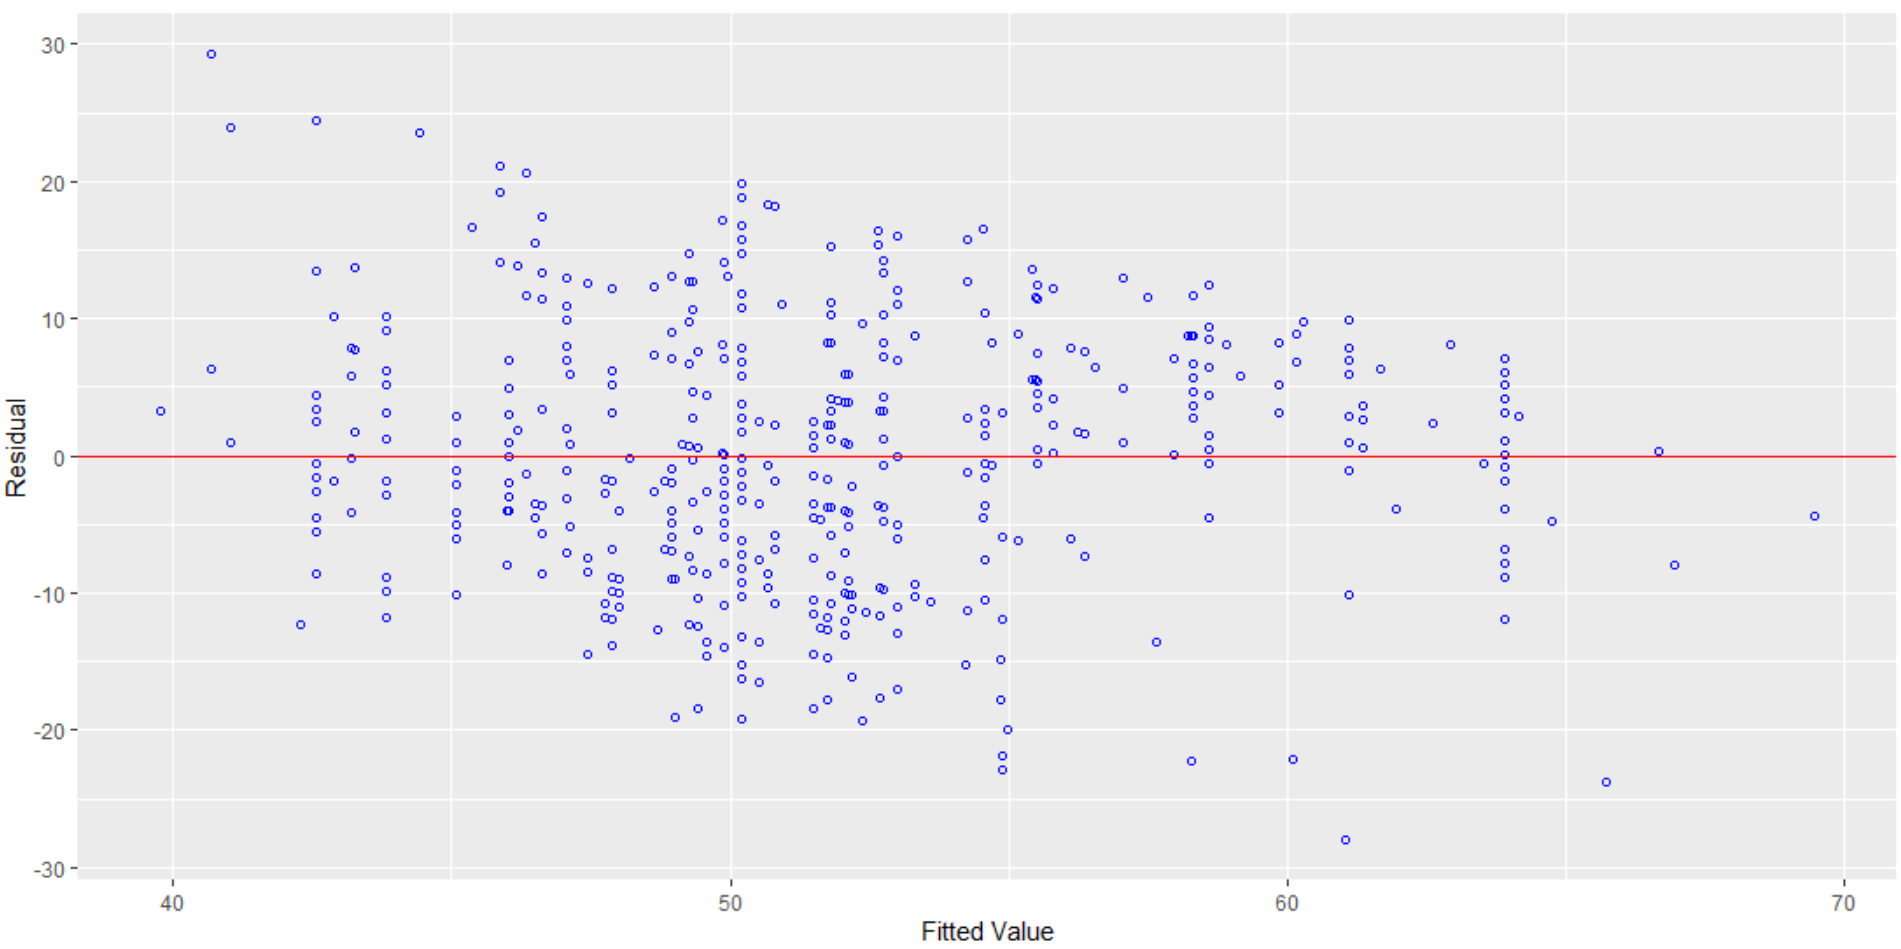
\includegraphics[width=0.9\textwidth]{graphiques/residus_VS_predicitions_lm1}
	\caption{Résidus en fonction des valeurs prédites pour le modèle \eqref{lm_1}.}
	\label{residus_VS_predicitions_lm1}
\end{figure}

\begin{figure}[H]  % residus_VS_predicitions_lm3_Qst1a
	\centering
	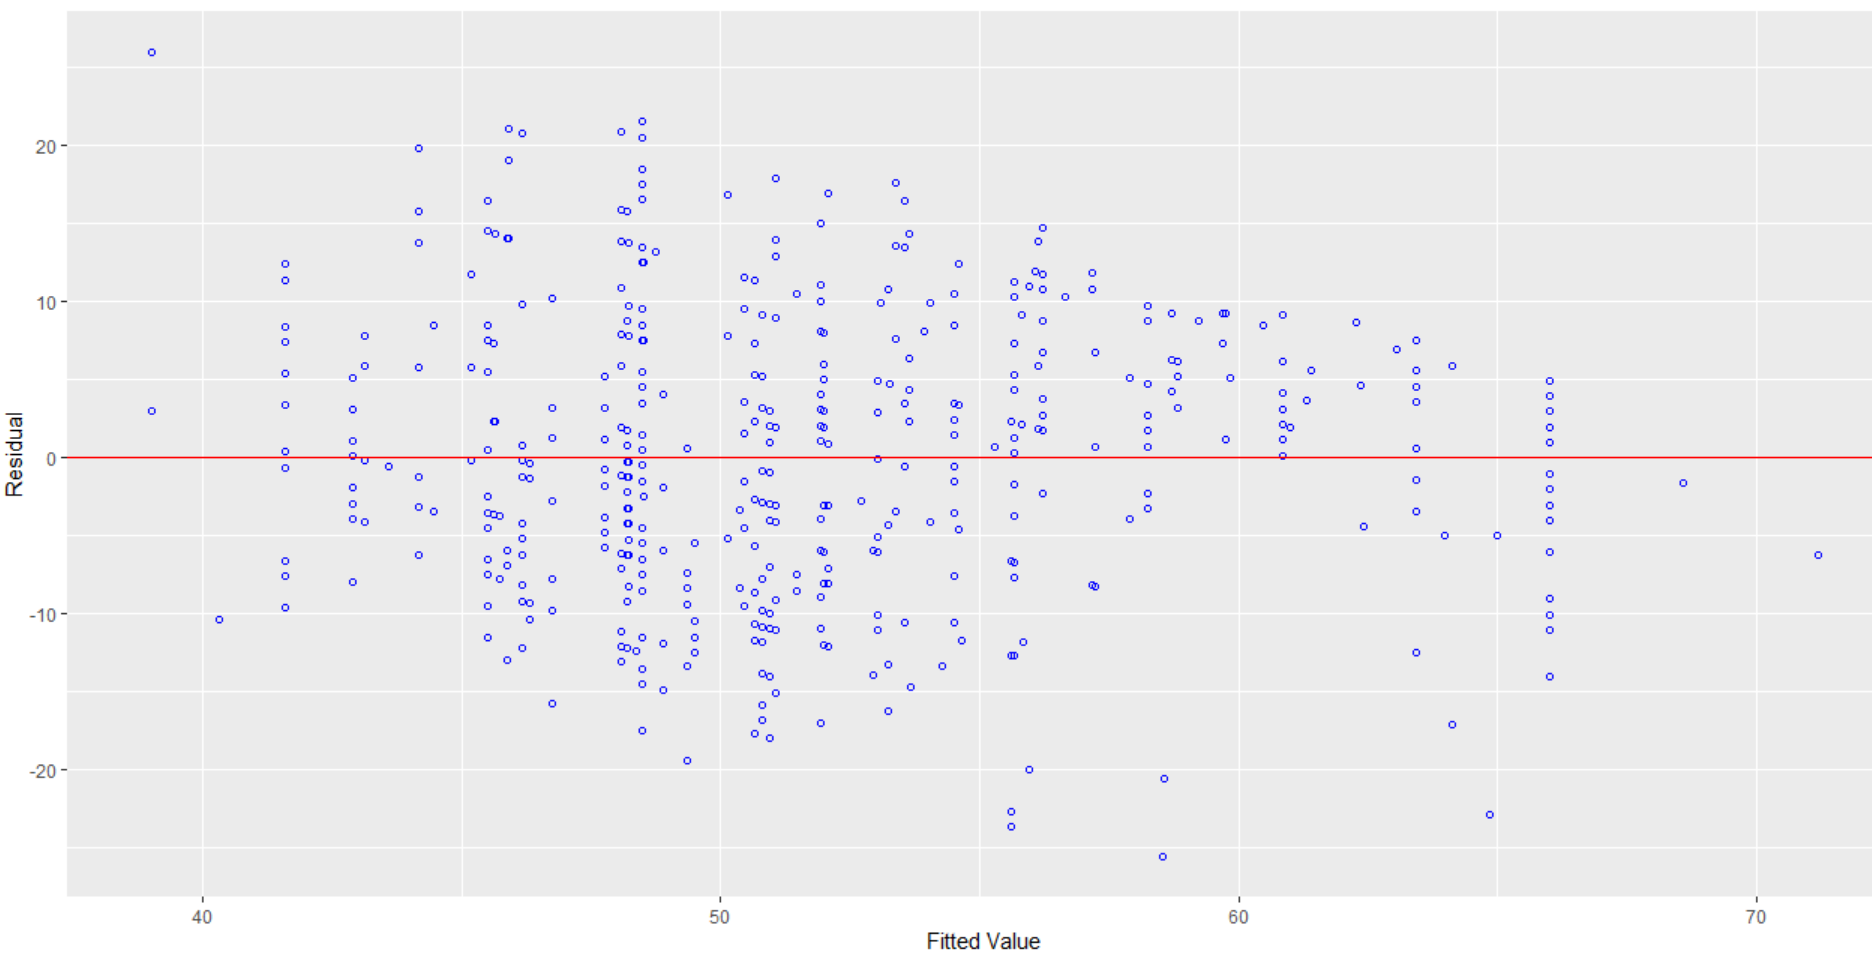
\includegraphics[width=0.9\textwidth]{graphiques/residus_VS_predicitions_lm2}
	\caption{Résidus en fonction des valeurs prédites pour le modèle \eqref{lm_3}.}
	\label{residus_VS_predicitions_lm3}
\end{figure}

\begin{figure}[H]  % residus_VS_predicitions_lm_Qst1b
	\centering
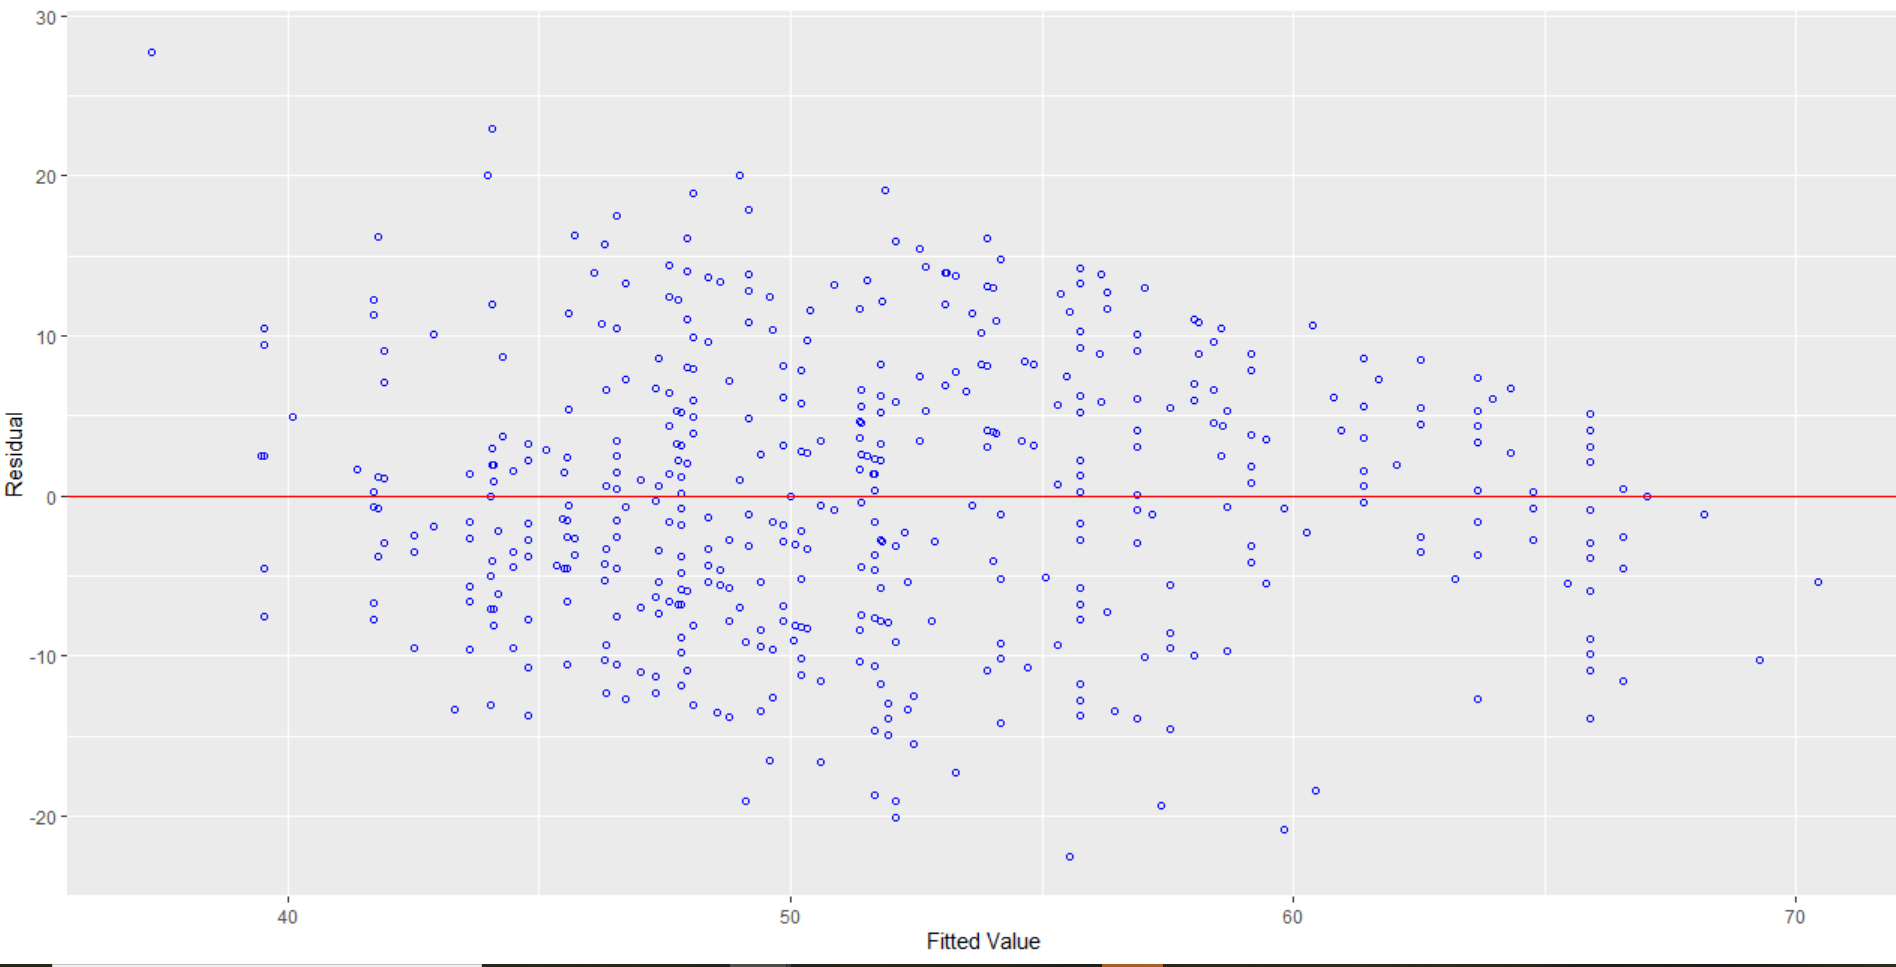
\includegraphics[width=0.9\textwidth]{graphiques/residus_VS_predicitions_lm_Qst1b}
\caption{Résidus en fonction des valeurs prédites pour le modèle \eqref{lm_qst1b}.}
\label{residus_VS_predicitions_lm_Qst1b}
\end{figure}

\begin{figure}[H]  % Spline_lm1
	\centering
	\begin{subfigure}{0.48\textwidth}
		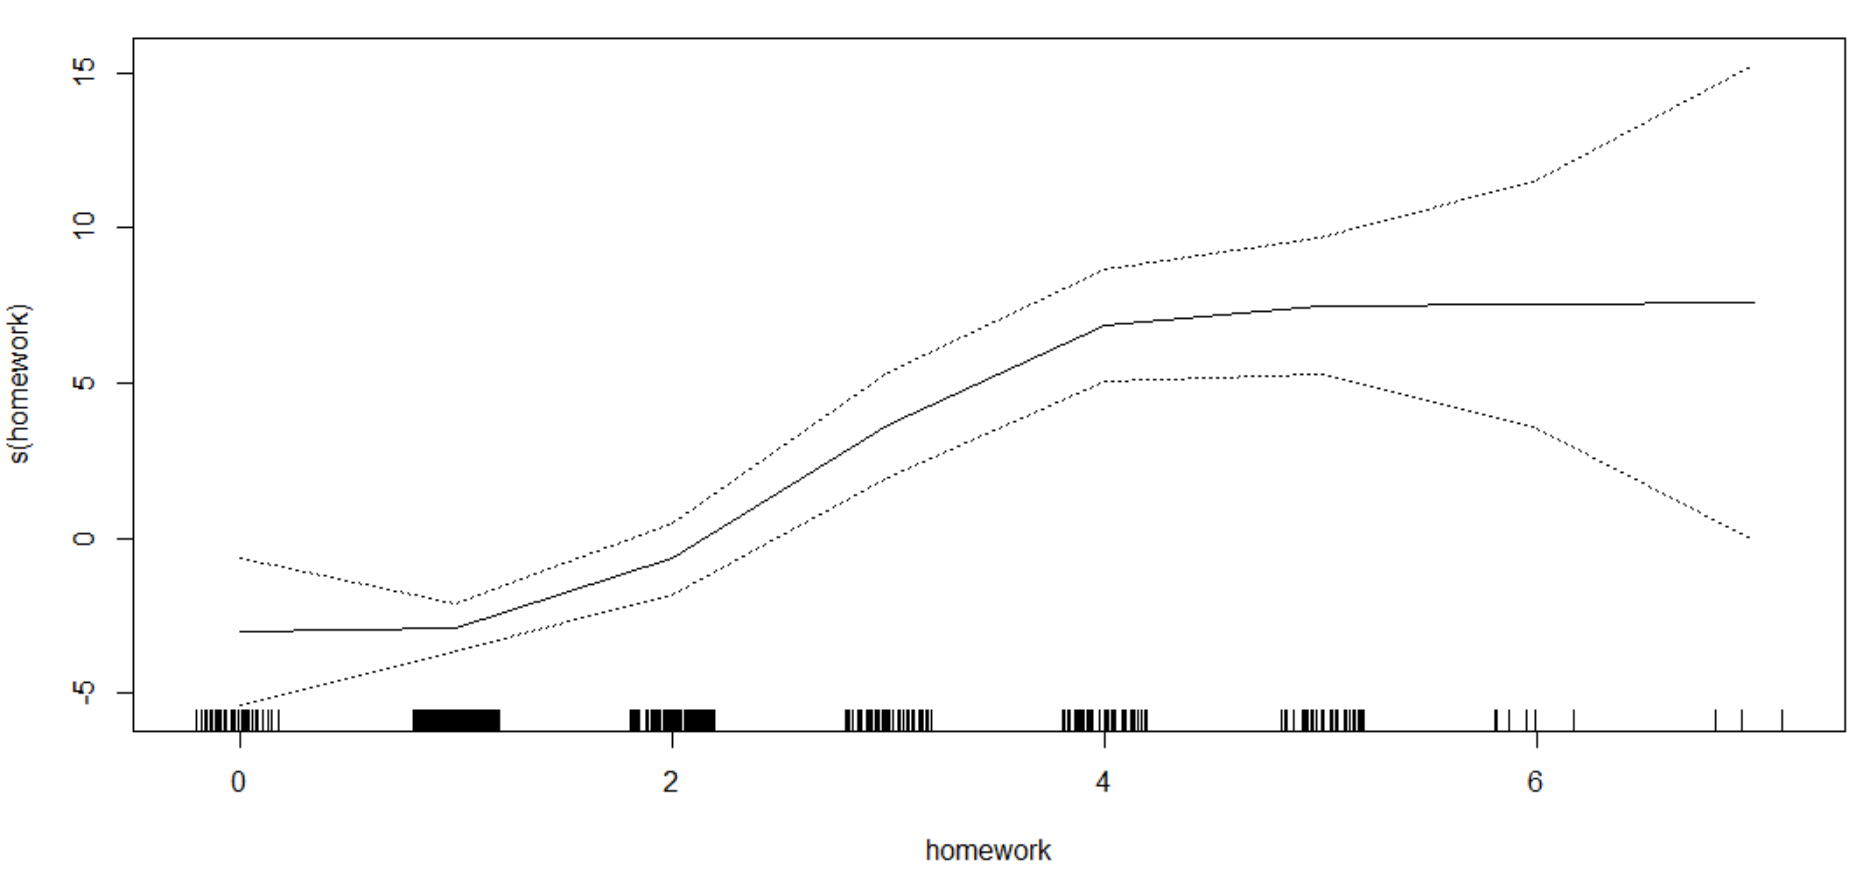
\includegraphics[width=1\textwidth]{graphiques/Spline_Homework}
		\caption{\texttt{homework}}
		\label{Spline_Homework}
	\end{subfigure}
	\begin{subfigure}{0.48\textwidth}
		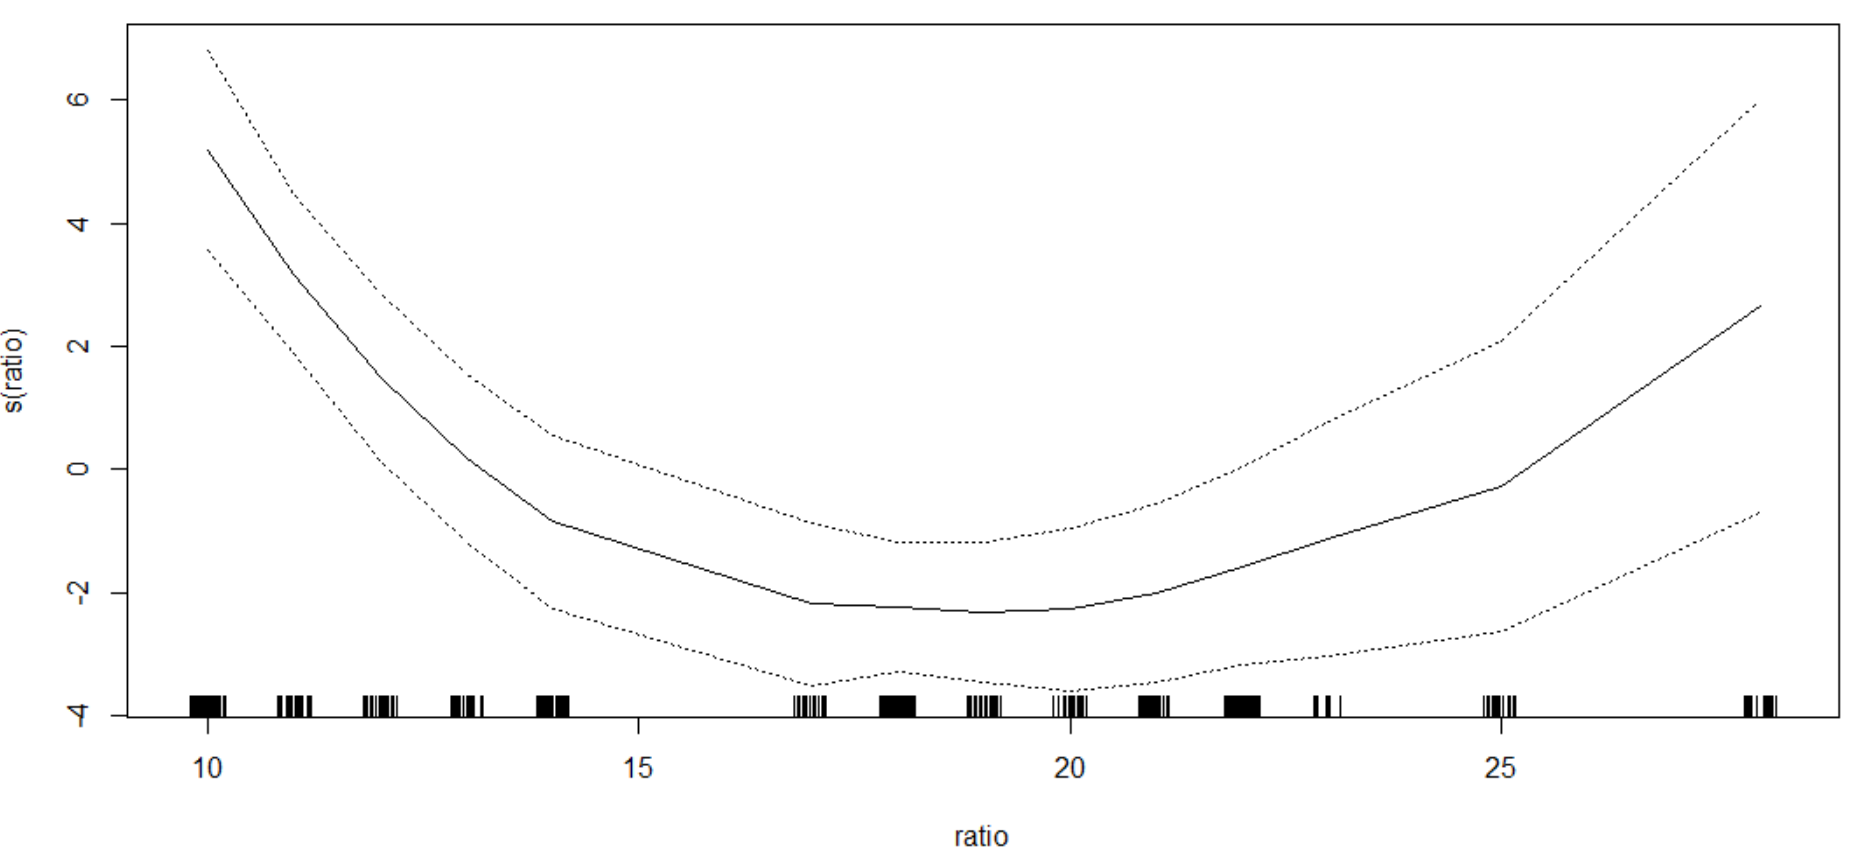
\includegraphics[width=1\textwidth]{graphiques/Spline_Ratio}
		\caption{\texttt{ratio}}
		\label{Spline_Ratio}
	\end{subfigure}
	\caption{Splines réalisés sur les variables \texttt{homework} et \texttt{ratio} lors de l'entraînement d'un GAM.}
	\label{Spline_lm1}
\end{figure}

\begin{figure}[H]  % Spline_lm2
	\centering
	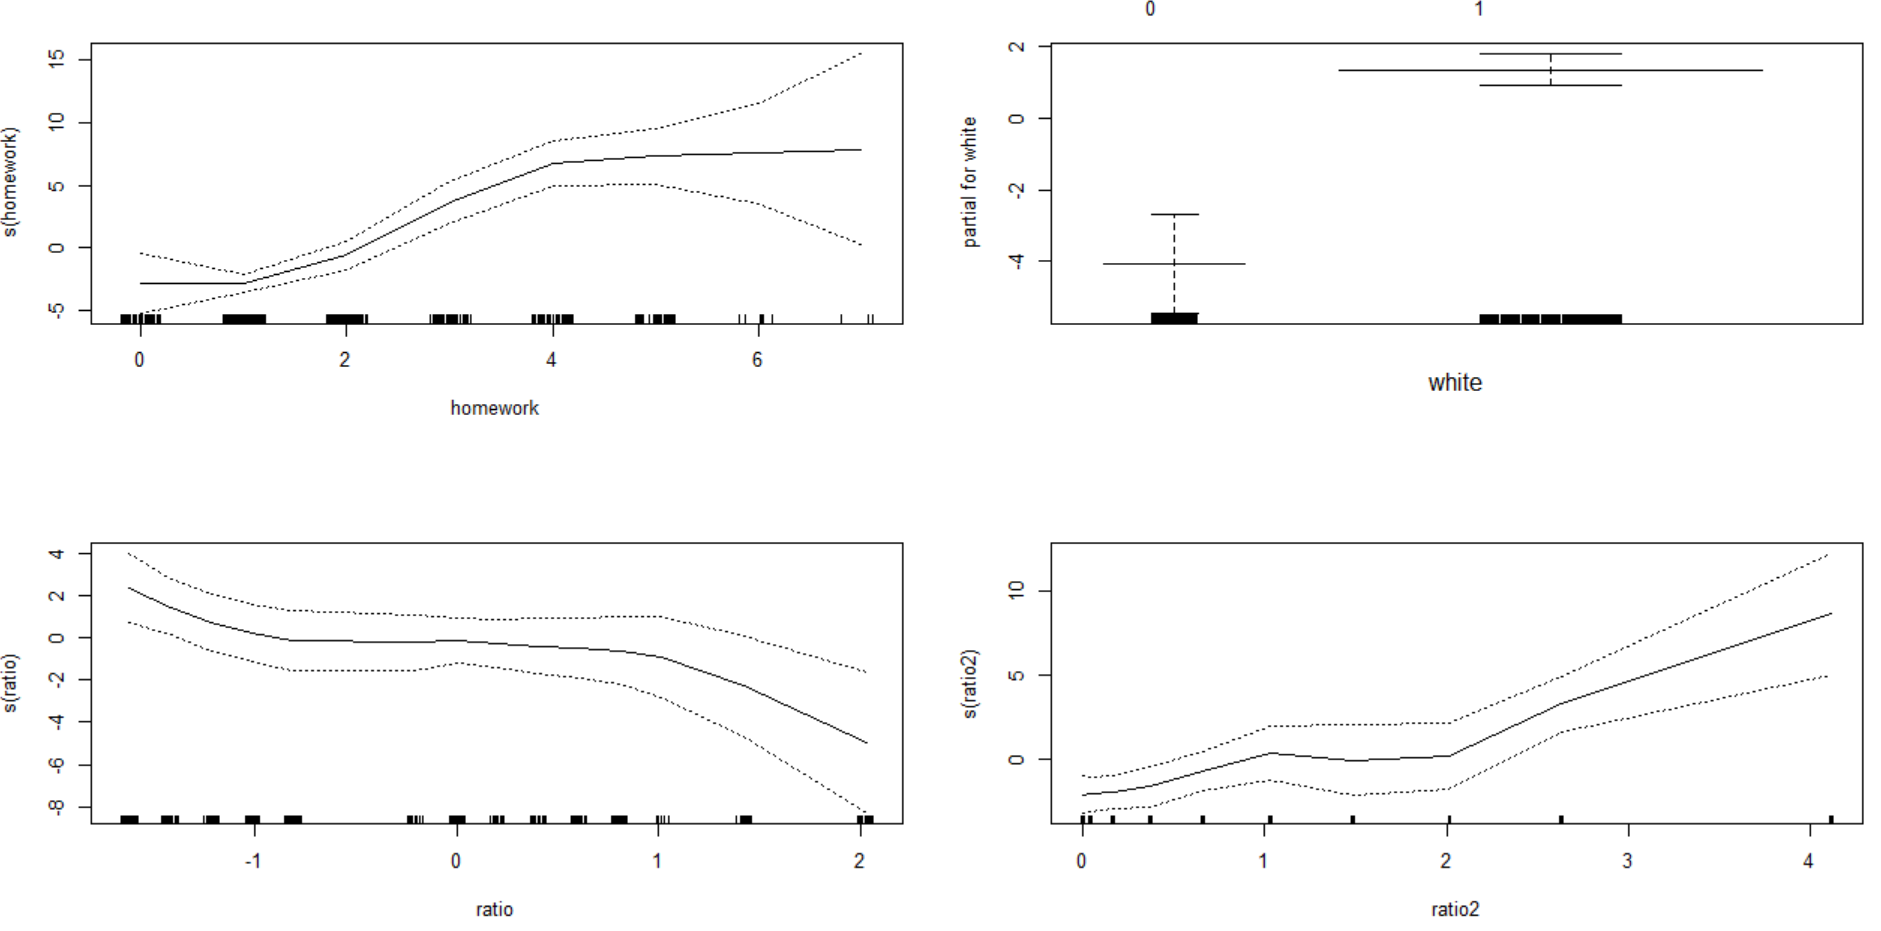
\includegraphics[width=1\textwidth]{graphiques/Splines2}
	\caption{Visualisation des Splines suite à l'entraînement d'un GAM utilisant \eqref{lm_2}.}
	\label{Spline_lm2}
\end{figure}

\begin{figure}[H]  % residus_VS_id_qst1a
	\centering
	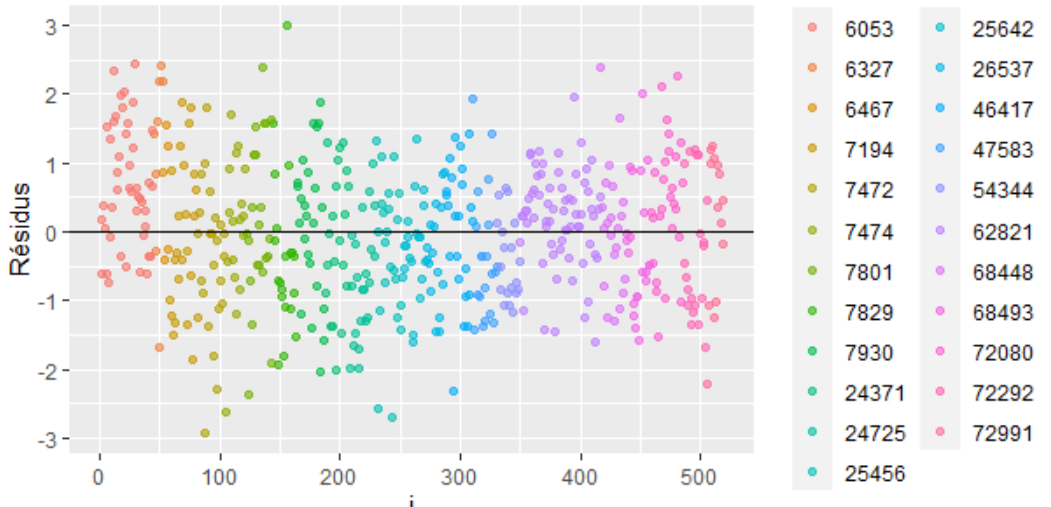
\includegraphics[width=0.9\textwidth]{graphiques/residus_VS_id_qst1a}
	\caption{Résidus studentisés en fonction de l'index des observations pour le modèle \ref{lm_3}.}
	\label{residus_VS_id_qst1a}
\end{figure}

\begin{figure}[H]  % residus_VS_id_qst1b
	\centering
	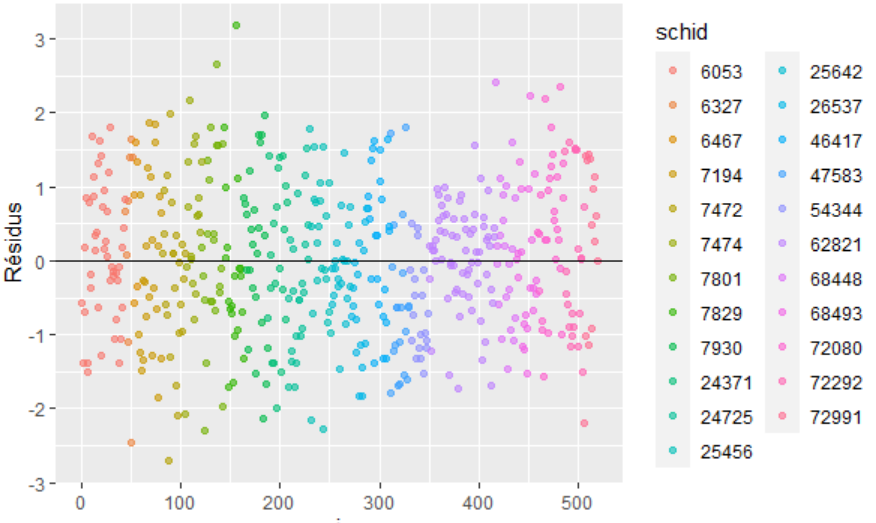
\includegraphics[width=0.9\textwidth]{graphiques/residus_VS_id_qst1b}
	\caption{Résidus studentisés en fonction de l'index des observations pour le modèle \ref{lm_qst1b}.}
	\label{residus_VS_id_qst1b}
\end{figure}

\begin{figure}[H]  % Residus_VS_variables_qst1a
	\centering
	\begin{subfigure}{0.48\textwidth}
		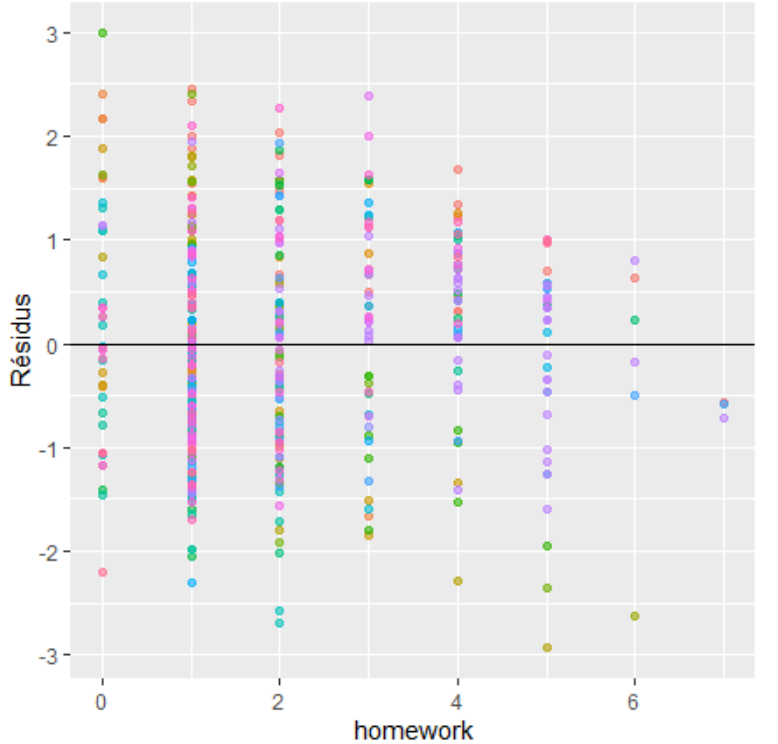
\includegraphics[width=1\textwidth]{graphiques/Residus_VS_Homework}
		\caption{\texttt{homework}}
		\label{Residus_VS_Homework}
	\end{subfigure}
	\begin{subfigure}{0.48\textwidth}
		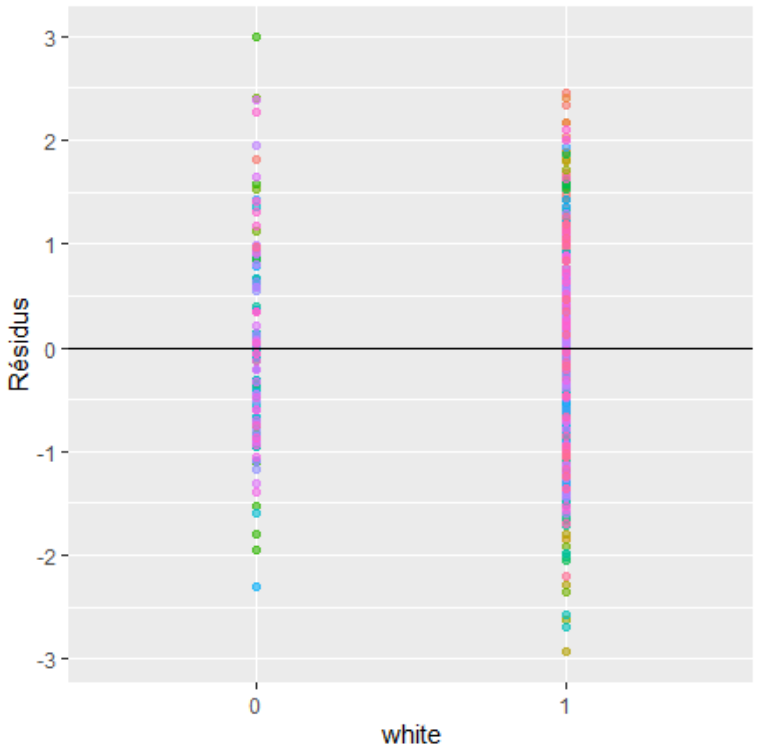
\includegraphics[width=1\textwidth]{graphiques/Residus_VS_white}
		\caption{\texttt{white}}
		\label{Residus_VS_white}
	\end{subfigure}
	\begin{subfigure}{0.48\textwidth}
		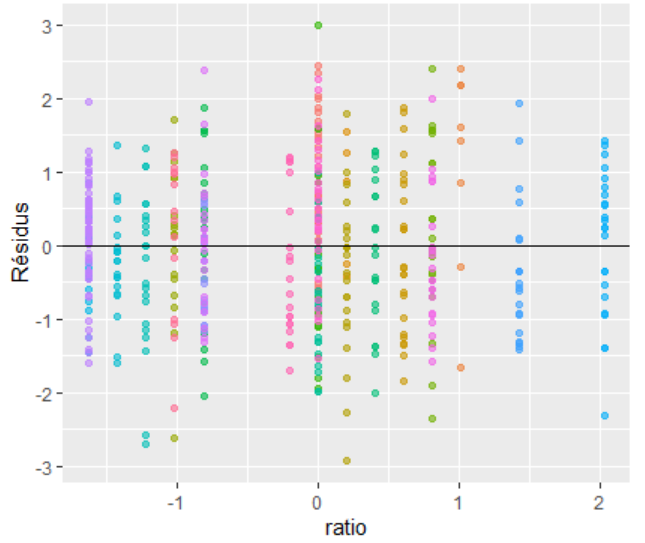
\includegraphics[width=1\textwidth]{graphiques/Residus_VS_ratio}
		\caption{\texttt{ratio}$^*$}
		\label{Residus_VS_ratio}
	\end{subfigure}
	\begin{subfigure}{0.48\textwidth}
		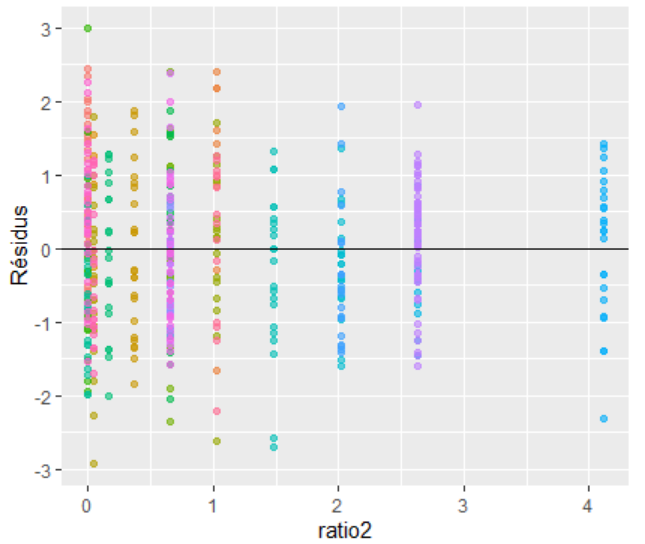
\includegraphics[width=1\textwidth]{graphiques/Residus_VS_ratio2}
		\caption{\texttt{ratio2}}
		\label{Residus_VS_ratio2}
	\end{subfigure}
	\caption{Résidus studentisés en fonction des différentes variables explicatives du modèle \ref{lm_3}.}
	\label{Residus_VS_variables_lm3}
\end{figure}

\begin{figure}[H]  % Residus_VS_variables_qst1b
	\centering
	\begin{subfigure}{0.48\textwidth}
		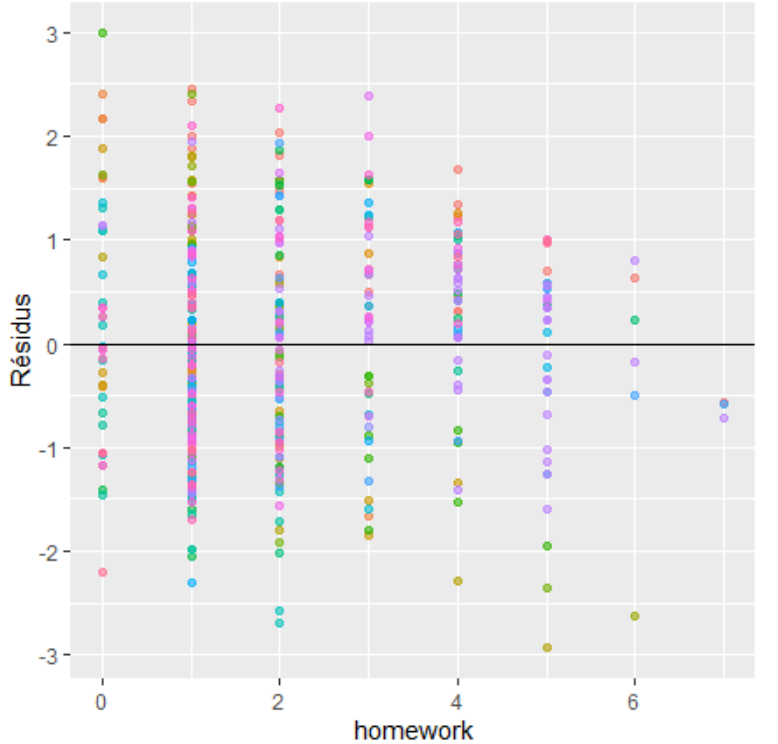
\includegraphics[width=1\textwidth]{graphiques/Residus_VS_Homework}
		\caption{\texttt{homework}}
		\label{Residus_VS_Homework_qst1b}
	\end{subfigure}
	\begin{subfigure}{0.48\textwidth}
		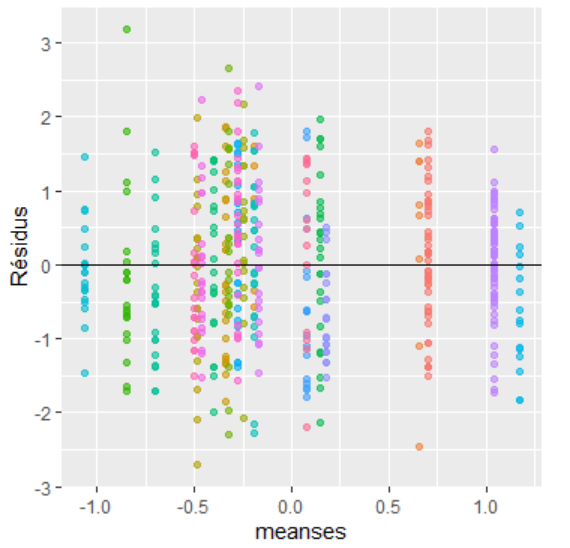
\includegraphics[width=1\textwidth]{graphiques/Residus_VS_meanses}
		\caption{\texttt{meanses}}
		\label{Residus_VS_meanses}
	\end{subfigure}
	\begin{subfigure}{0.48\textwidth}
		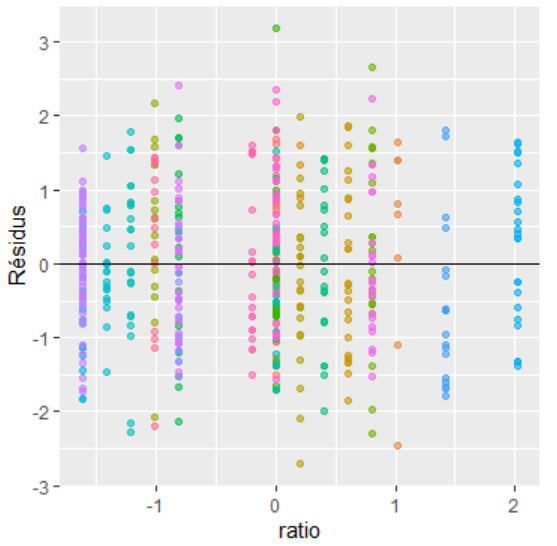
\includegraphics[width=1\textwidth]{graphiques/Residus_VS_ratio_qst1b}
		\caption{\texttt{ratio}$^*$}
		\label{Residus_VS_ratio_qst1b}
	\end{subfigure}
	\begin{subfigure}{0.48\textwidth}
		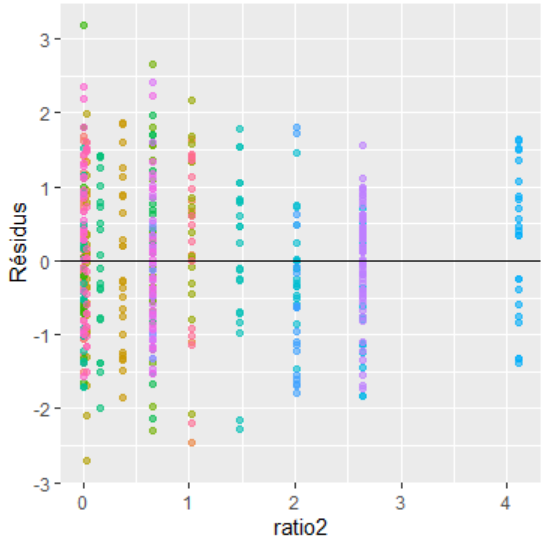
\includegraphics[width=1\textwidth]{graphiques/Residus_VS_ratio2_qst1b}
		\caption{\texttt{ratio2}}
		\label{Residus_VS_ratio2_qst1b}
	\end{subfigure}
	\caption{Résidus studentisés en fonction des différentes variables explicatives du modèle \ref{lm_qst1b}.}
	\label{Residus_VS_variables_qst1b}
\end{figure}

\begin{figure}[H]  % summary_Qst1a
	\centering
	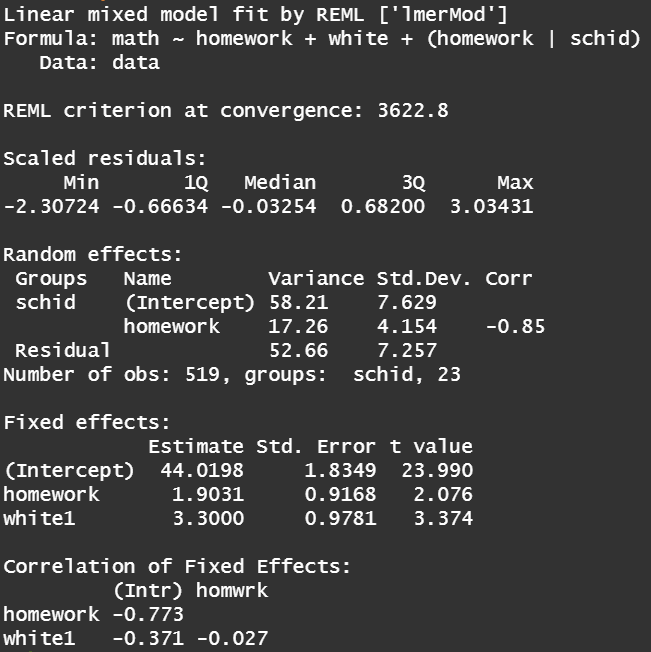
\includegraphics[width=0.5\textwidth]{graphiques/summary_Qst1a}
	\caption{Sortie \texttt{R} de la fonction \texttt{summary} pour le modèle \eqref{lmm_qst1a}.}
	\label{summary_Qst1a}
\end{figure}

\begin{figure}[H]  % summary_Qst1b
	\centering
	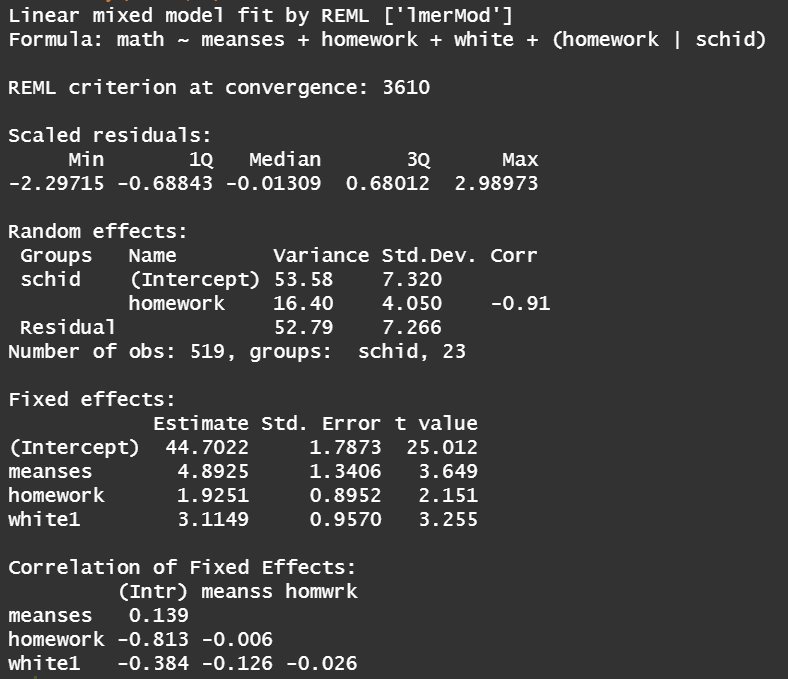
\includegraphics[width=0.6\textwidth]{graphiques/summary_Qst1b}
	\caption{Sortie \texttt{R} de la fonction \texttt{summary} pour le modèle \eqref{lmm_qst1b}.}
	\label{summary_Qst1b}
\end{figure}


\subsection{Question 2}

\begin{figure}[H]  % Grandeur_VS_age_Qst2
	\centering
	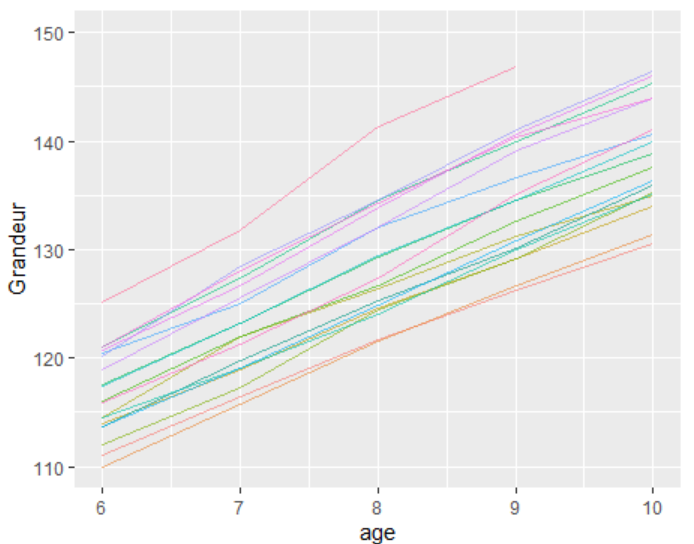
\includegraphics[width=0.6\textwidth]{graphiques/Grandeur_VS_age_Qst2}
	\caption{Relation de la grandeur en fonction de l'âge pour chacune des jeunes filles.}
	\label{Grandeur_VS_age_Qst2}
\end{figure}
	
\begin{figure}[H]  % Residus_qst2
	\centering
	\begin{subfigure}{0.48\textwidth}
		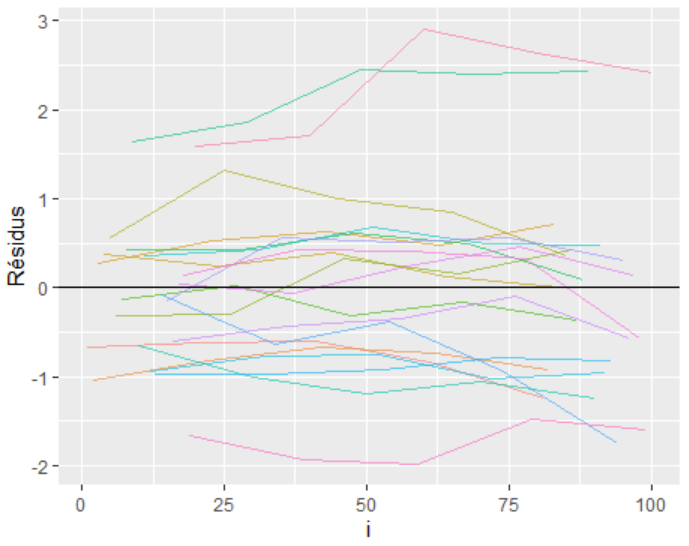
\includegraphics[width=1\textwidth]{graphiques/residus_VS_id_qst2}
		\caption{\texttt{i}}
		\label{residus_VS_id_qst2}
	\end{subfigure}
	\begin{subfigure}{0.48\textwidth}
		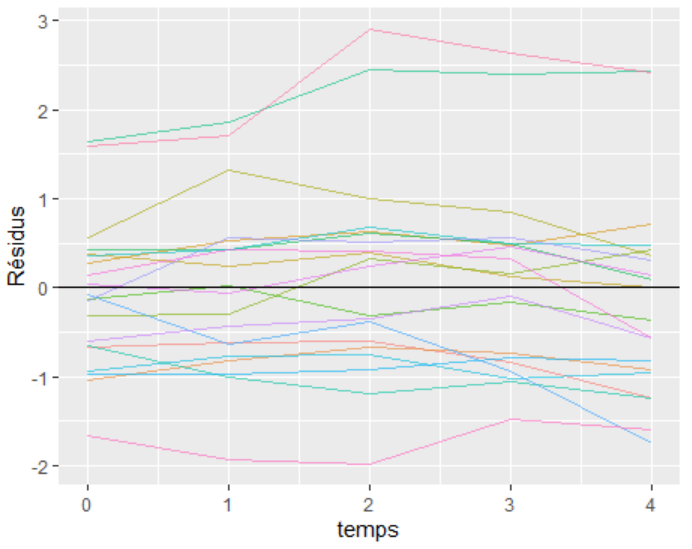
\includegraphics[width=1\textwidth]{graphiques/Residus_VS_temps_qst2}
		\caption{\texttt{temps}}
		\label{Residus_VS_temps_qst2}
	\end{subfigure}
	\begin{subfigure}{0.48\textwidth}
		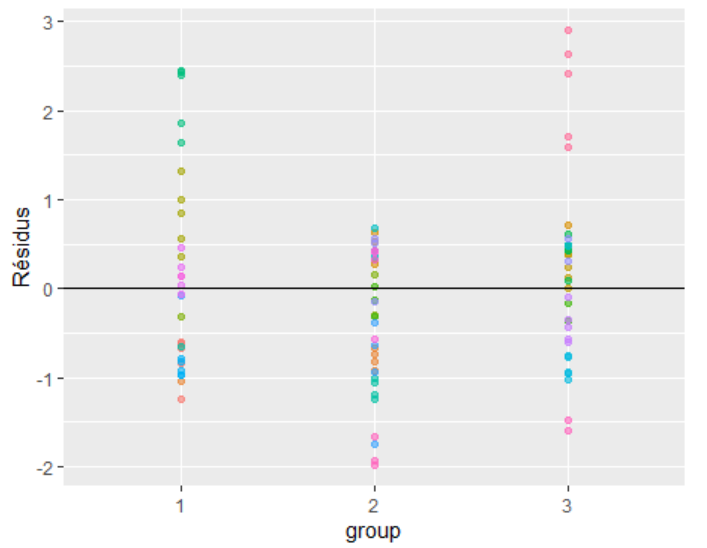
\includegraphics[width=1\textwidth]{graphiques/Residus_VS_group_qst2}
		\caption{\texttt{group}}
		\label{Residus_VS_group_qst2}
	\end{subfigure}
	\caption{Graphiques de résidus générés à partir du modèle \eqref{lm_qst2}.}
	\label{residus_qst2}
\end{figure}

\begin{figure}[H]  % summary_Qst2
	\centering
	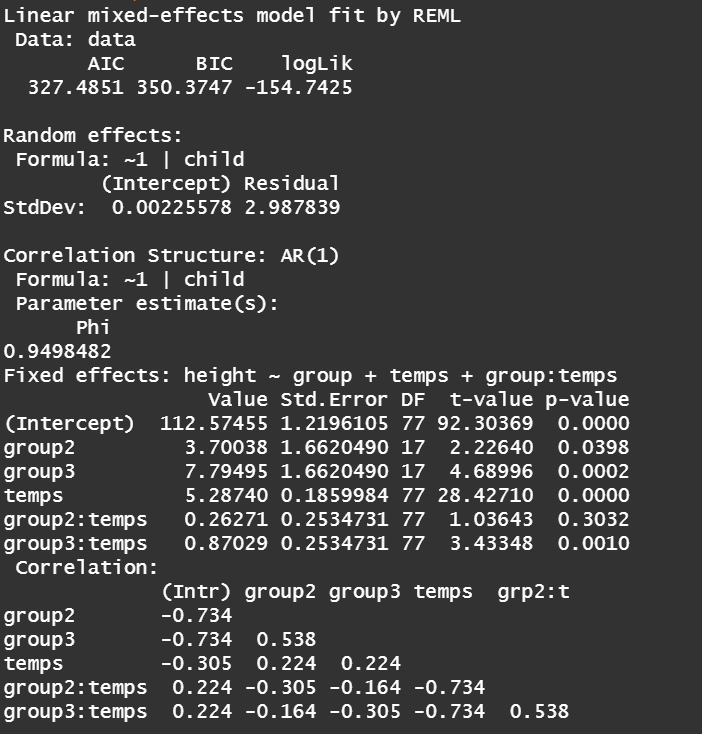
\includegraphics[width=0.6\textwidth]{graphiques/summary_Qst2}
	\caption{Sortie \texttt{R} de la fonction \texttt{summary} pour le modèle \eqref{lmm_qst2_final}.}
	\label{summary_Qst2}
\end{figure}


\subsection{Question 3}

	
\end{document}